\documentclass[a4j,dvipdfmx]{jsarticle}

\usepackage[dvipdfmx]{graphicx}
\usepackage{amsmath,amssymb}
\usepackage{siunitx}
\usepackage{ascmac}
\usepackage[subrefformat=parens]{subcaption}
\usepackage{fancyhdr}
\usepackage{otf}
\usepackage[dvipdfmx]{hyperref}
\usepackage{pxjahyper}
\usepackage{okumacro}


\pagestyle{headings}

% \renewcommand{\thesubsection}{\arabic{subsection}}
\renewcommand{\headrulewidth}{1pt}
\renewcommand{\Re}{\operatorname{Re}}
\renewcommand{\Im}{\operatorname{Im}}


\newcounter{basic_quastion}\setcounter{basic_quastion}{1}
\newcommand{\basicquestion}{\noindent{\large 基本問題\hspace{1mm}\huge\fbox{\textbf{\arabic{basic_quastion}}}\addtocounter{basic_quastion}{1}}\thispagestyle{fancy}\lhead{$\Sigma$基本問題}\rhead{\thepage}\cfoot{}\quad}
\newcommand{\sign}{\mathop{\mathrm{sign}}\nolimits}
\newcommand{\linktoMOKUZI}{\vspace{\stretch{1}}\fbox{\centerline{\hyperref[目次]{目次に戻る}}}}

\newcounter{basic_answer}\setcounter{basic_answer}{1}
\newcommand{\basicanswer}{\noindent{\large 基本問題\hspace{1mm}\huge\fbox{\textbf{\arabic{basic_answer}}}\addtocounter{basic_answer}{1}}\thispagestyle{fancy}\lhead{基本問題解答}\rhead{\thepage}\cfoot{}\quad}



\title{Quuノート ー微分積分\ajRoman{1}ー}
\date{最終更新 2023/12/01}
\author{責任者 Quu}

\begin{document}
    \maketitle
    \thispagestyle{empty}
    \begin{figure}[h]
        \centering
        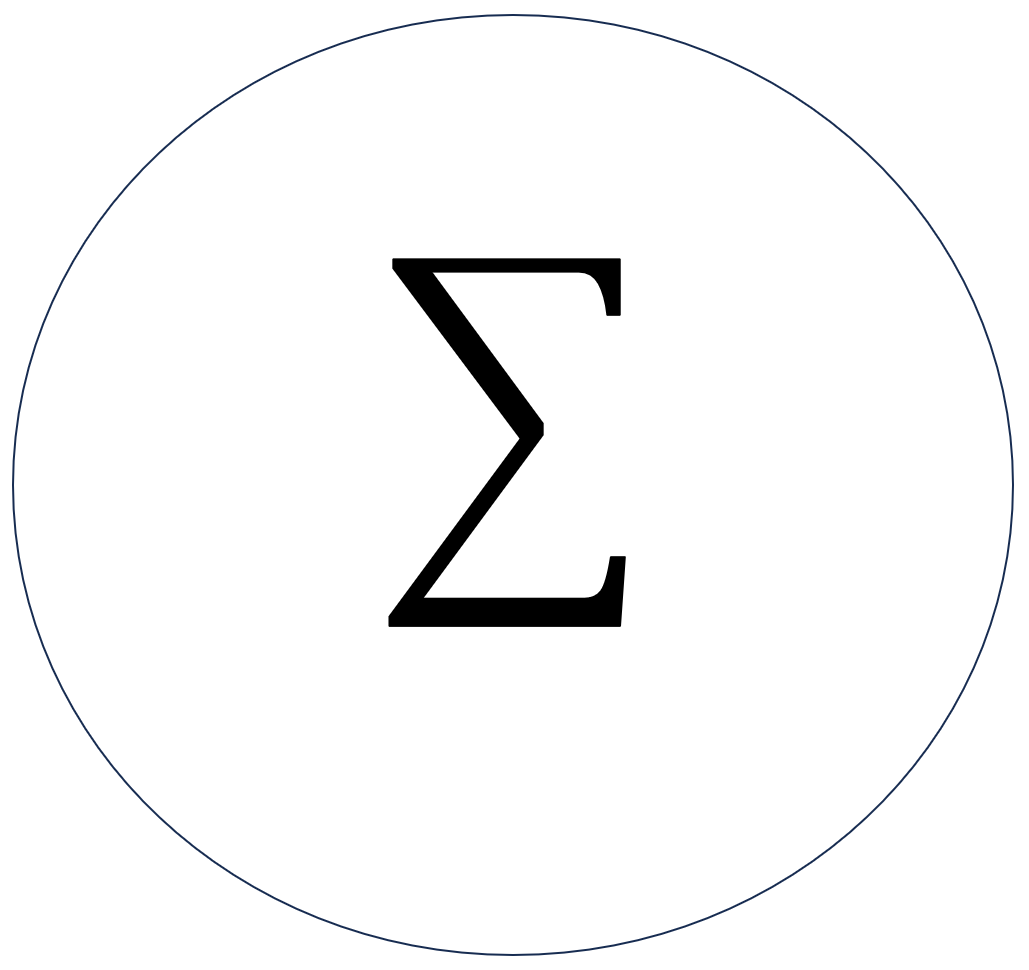
\includegraphics[scale=0.5]{img/QuuNote/icon.png}
    \end{figure}
    
    \vspace{\stretch{1}}
    \centerline{\textbf{概要}}
    \noindent
    微分積分学入門についてのノート。\\
    主に、一変数の極限、一変数の微分・積分、実数の無限級数について扱う。
    
    \clearpage
    \label{目次}
    \tableofcontents
    \clearpage
    
    \part{前提知識}
    \vspace{\stretch{1}}
    \begin{screen}
        微分積分を学ぶうえで前提となる知識をまとめた。微分積分は主に関数の微分・積分について扱うわけだから、ある程度の関数の扱い方も知っておく必要がある。
        そのほか数の種類についてや閉区間・開区間、極限についてもまとめてある。極限は微分積分を学ぶ際にいたるところに出てきて、陰から支える縁の下の力持ち的な役割を持つ。極限は一見すると
        代入と同じように見えるが、実は違う。極限は代入だと都合が悪い時にありがたみが実感できる。極限に関連して、無限という概念も登場する。
    \end{screen}
    \clearpage
    \section{様々な`数'と数直線}
        \subsection{数の種類}
            数学を勉強するうえで、様々な数が登場する。まず一番初めに思いつくのが$1,2,3...$といった\textbf{自然数}である。
            次の自然数に$0$と負の符号をつけたものを加えた\textbf{整数}が考えられる。整数同士で足し算、引き算、掛け算を行っても
            その値は整数である。このことを\textbf{和、差、積について閉じている}という。これは$a,b\in \mathbb{Z}$となる任意の$a,b$
            について
            \begin{equation}
                a+b , a-b , a\times b \in \mathbb{Z}
            \end{equation}
            が成り立つことを意味している。

            一方割り算は整数の中に閉じていない。\footnote{例えば$1\div 2$など。}しかし、$0.5,3.14$などの\textbf{有理数}まで数を拡張すれば、その中に商は閉じている。
            つまり、$a,b \in \mathbb{Q}$となる任意の$a,b$について
            \begin{equation}
                \frac{a}{b} \in \mathbb{Q}
            \end{equation}
            となる。よって、数を有理数まで拡張すれば\textbf{四則について閉じている}ことがわかる。

            さらに数の拡張を考えよう。たとえば$x^2-2=0$を満たす$x$について考えてみるには、数を\textbf{無理数}まで拡張しなければならない。
            一般の二次方程式の解も
            \begin{equation}
                x = \frac{-b\pm \sqrt{b^2-4ac}}{2a}
            \end{equation}
            と有理数だけでは表現できないことがわかる。無理数には$\pi,e\footnote{自然対数の底またはネイピア数と呼ばれる。具体的な値は$e=2.71...$}$などの\textbf{超越数}もふくむ。

            私たちの生活の中では有理数と無理数をあわせた\textbf{実数}があれば十分事足りるが、数学の世界ではそうもいかない。先ほどの二次方程式についてより深く調べてみると、
            解を持たない条件(根号の中身が負)があることがすぐに分かる。例えば、$x^2+1 = 0$は$x^2 = -1$と変形できるが、二乗して負になるような数は実数のうちには存在しない。
            よってこの方程式は\textbf{解なし}となる。がしかし、ここで
            \begin{equation}
                i = \sqrt{-1}
            \end{equation}
            となる`数'を定義してあげると、方程式は$x=\pm i$となり、$(実数)+i$を含めた範囲に解をもつことがわかる。
            この数は、今までの実数とは異なる数であり、実数との和,差は直接計算できない。一般に実数$a,b$と$i$を用いて
            \begin{equation}
                z = a + bi
            \end{equation}
            として表した$z$を\textbf{複素数}といい、$i$を虚数単位という。さらに$a$を$z$の実部、$b$を$z$の虚部といい、それぞれ
            $a=\Re z,b=\Im z$と表す。

            先ほど、二次方程式の解を有理数だけでは表現できないといったが、実は無理数を含めてもできない。この複素数を含めることで初めてすべて表現できるようになるのだ。\footnote{もちろんこれで数の拡張が終わるわけではない。しかし微分積分を学ぶうち間は複素数まで拡張すれば事足りる。}
        \subsection{数直線}
            では、数の大小関係をわかりやすくするためにはどうすればよいだろうか。視覚的にわかりやすくするためには数直線を用いればよい。
            \begin{figure}[h]
                \centering
                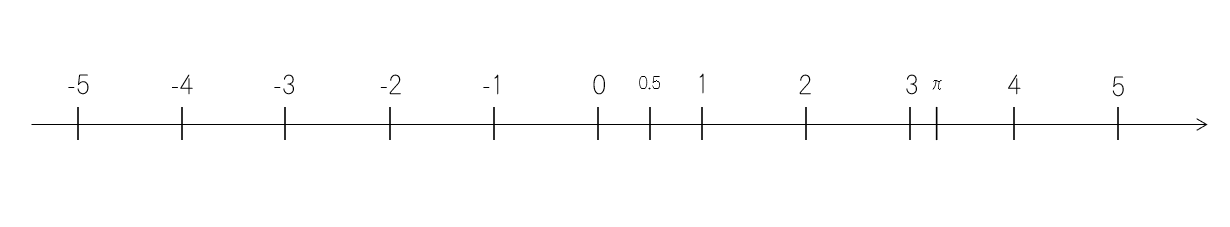
\includegraphics[keepaspectratio,scale=0.5]{img/QuuNote/NumLine_1.png}
                \caption{数直線}
            \end{figure}
            
            上の例では、整数、有理数、無理数の一部を記載している。当然書いてある数以外も数直線の中には含まれている。
            むしろ、数の点の集まりとして数直線を捉える方がイメージがわきやすいかもしれない。
            ここで注意しなければならないのは、この数直線上に複素数$(\Im z\neq 0)$は含まれないといけないということである。
            数直線は\underline{実数を表す}直線なので、実数より(集合的に)大きい複素数のすべては含むことができないのである。

            では実数も含めた複素数はどう表せばよいのか。答えは単純で実数の軸\footnote{これを実軸と呼ぶ。}とは別の軸\footnote{虚軸という。}を
            加えればよい。つまり複素数は平`面'上で表せられるのである。\footnote{この平面を複素平面という。いつものy-xグラフとは見た目は同じだが感覚が違うので注意。}  
            \newpage
        \subsection{開区間・閉区間}
            実数が数直線上の一点で表せることはすでに前項で述べた。では点に続いて次は区間について考えていこう。

            区間は大きく二つある。それらはそれぞれ\textbf{開区間}、\textbf{閉区間}と呼ばれる。これらの違いは端点を含むかどうかで、
            逆に言えば端以外は同じである。例えば、$1<x<2,1\leq x\leq2$について前者は端点$x=1,2$を含まず、後者は端点を含むのである。
            端点を含まない場合が開区間、端点を含む場合が閉区間である。

            閉区間、開区間を数直線上で表すにはどうすればよいだろうか。これも数直線と同様に区間の端から端まで線を引けばよい。注意しないといけないのが
            端点で、区間が開区間か閉区間かによって端点を書き分けないといけない。開区間のときは$\circ$、閉区間のときは$\bullet$と書けばよい。

            \begin{figure}[h]
                \centering
                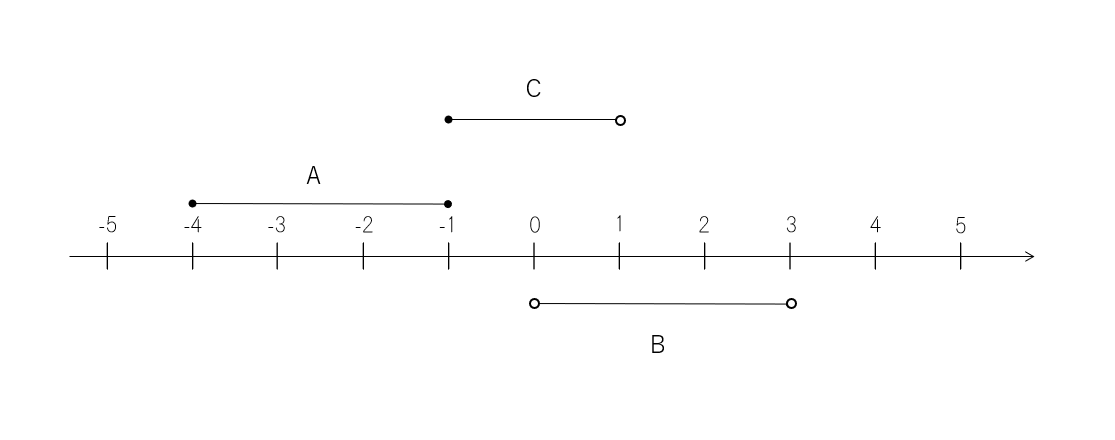
\includegraphics[keepaspectratio,scale=0.7]{img/QuuNote/IntervalLine.png}
                \caption{開区間と閉区間}
            \end{figure}
            例えば上図の例をみてみると、$A,B,C$の三つの区間がある。それぞれ$-4\leq x\leq -1,0<x<3,-1\leq x<1$となる。
            今までは不等号を用いて区間を表現してきたが\footnote{厳密に言えば区間は集合なので、不等号を用いて区間を表現するという言い方は適切ではない。}、もっと簡潔に$(\hspace{1mm}),[\hspace{1mm}]$を用いて表現する方法もある。
            この表現方法を使えば、$A,B,C$はそれぞれ$[-4,-1],(0,3),[-1,1]$と表せる。$(\hspace{1mm})$が等号を含まない、$[\hspace{1mm}]$が
            等号を含む、というわけである。

            では、値が無限に続く(例えば実数全体など)場合はどう表現すればよいのか。この場合は無限大の記号$\infty$を用いて$(-\infty,\infty)$などと表せばよい。\footnote{この方法を使えば、a以上の実数などの場合でも$[a,\infty)$と表せばよいことがわかる。}
            \clearpage
            
        \basicquestion 以下問に答えよ。

        \paragraph{問1}以下の主張のうち正しいものには〇を、間違っているものには×をつけよ。
            \begin{enumerate}
                \item $\sqrt{9}$は無理数である。
                \item 有理数は全て分子分母が整数である分数の形で表せる。
                \item $i$は複素数である。
                \item 有理数の集合は$\mathbb{Q}$として表し、無理数の集合は$\mathbb{N}$で表す。
                \item 自然数全体の集合(区間)は$(0,\infty]$である。
            \end{enumerate}
        \paragraph{問2}以下の区間について、数直線上に示せ。もし数直線上に記されていない数字が出てくる場合はそれも記載せよ。
            \begin{figure}[h]
                \centering
                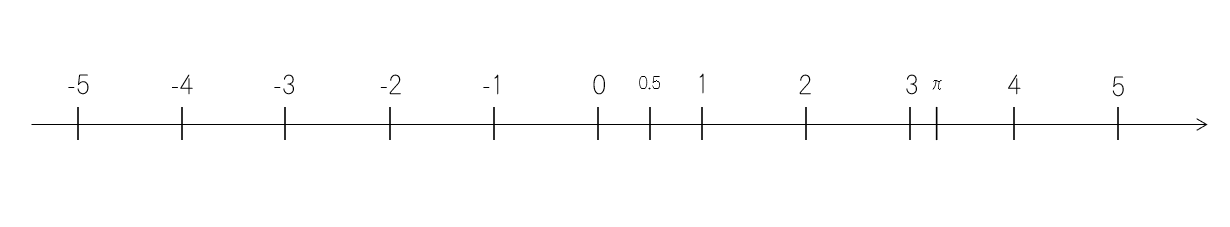
\includegraphics[keepaspectratio,scale=0.6]{img/QuuNote/NumLine_1.png}
                \caption{数直線}
            \end{figure}

            $1.\quad [2,3]$\hspace{3mm}
            $2.\quad (3,5)$\hspace{3mm}
            $3.\quad [-5,\pi]$\hspace{3mm}
            $4.\quad (-2,0.5]$\hspace{3mm}
            $5.\quad [-1,0)$\hspace{3mm}
            $6.\quad (-\infty,0)$\hspace{3mm}
            $7.\quad [0,\infty)$\hspace{3mm}
        \clearpage
        
        \section{関数の性質}
            \subsection{偶関数・奇関数}
                一般の関数$f(x)$について、$f(-x)=f(x)$を満たすものを\textbf{偶関数}、$f(-x)=-f(x)$を満たすものを\textbf{奇関数}という。
                もちろん全ての関数が偶関数・奇関数のどちらかであるというわけではない。しかし、全ての関数は偶関数と奇関数の和で表せられること
                が知られている。\\

                関数が偶関数・奇関数である場合のグラフはどうなるだろうか。まずは偶関数から考えてみると、定義より$x>0$と$x<0$の点において$f$は
                同じ値を取るわけであるから、グラフはy軸に対して対象になるはずである。つぎに奇関数について考えてみよう。これも定義より$x>0$と$x<0$の
                点において、$f$はx軸に対してそれぞれ対象に点を取るはずである。つまり、グラフは原点に対して点対象になるはずである。\\

                偶関数の例となる関数は、$x^2,\cos x,a(\text{定数関数})$などがあげられる。奇関数の例となる関数は、$x,\sin x,\tan x$などがあげられる。
                各自でグラフソフトなどでグラフを見てみるとよい。
            \clearpage
            \subsection{べき関数}
                関数のなかでもっともなじみやすいのが、$f(x)=x^n$であろう。例えば$x$は一次関数、$x^2$は二次関数と呼ばれる。
                別に$n$は自然数に限らなくてもよい。$x^{\frac{1}{2}}=\sqrt{x}$は指数が自然数ではないが、これもべき関数の一つである。
                $n$が自然数のうちは、関数の定義域について特別意識をする必要はない。しかし$n=\frac{1}{2}$などのように指数が有理数であったり、
                $n=-1$のように指数が負の値を取る場合には定義域に十分注意する必要がある。このように、一般に$f(x)=x^n$で表される関数を\textbf{べき関数}という。

                次に関数のグラフについて、グラフ描画ソフトを用いて数式を入力すると以下のようになる。
                \begin{figure}[h]
                    \centering
                    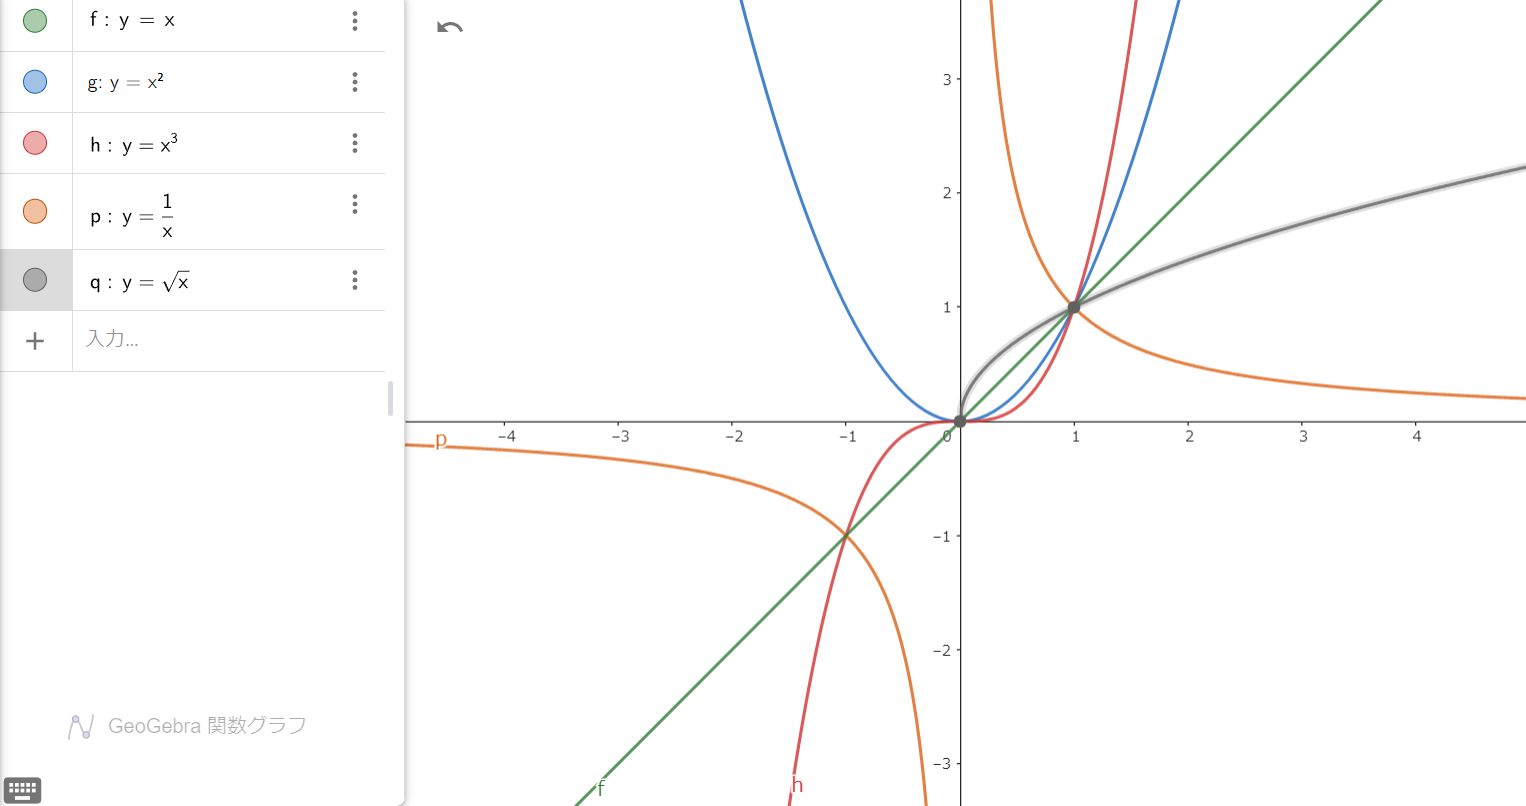
\includegraphics[keepaspectratio,scale=0.5]{img/QuuNote/PowerFuncGraph.png}
                    \caption{べき関数グラフ}
                \end{figure}

                図からも$\sqrt{x}$が$x<0$で定義されないことがわかる。また、$x^2$と$\sqrt{x}$は$y=x$を軸にして線対象になっており、
                $x^2$と$\sqrt{x}$は互いに\textbf{逆関数}であることがわかる。
            \clearpage
            \subsection{三角関数}
                \textbf{三角関数}は三角比を一般角に拡張した関数である。定義からわかるように周期関数であり、周期は$2\pi$である。
                三角比の定義自体を忘れた人はいないだろうが一応説明しておく。
                \begin{figure}[h]
                    \centering
                    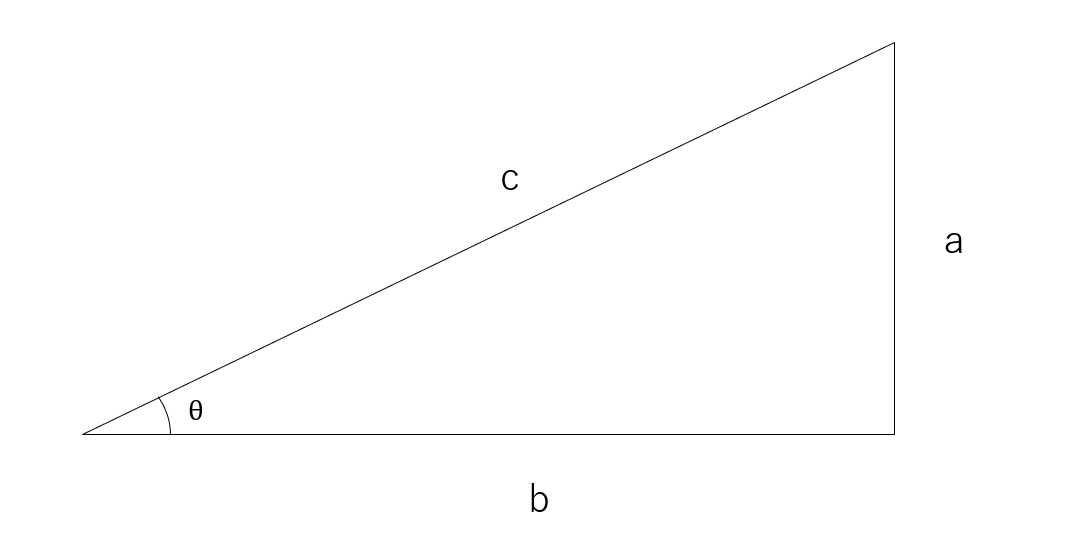
\includegraphics[keepaspectratio,scale=0.3]{img/QuuNote/triangleFunc.png}
                    \caption{三角比}
                \end{figure}

                上図\footnote{aの辺のことを対辺、bの辺のことを隣辺、cの辺のことを斜辺という。}において
                \begin{align}
                    \sin \theta &= \frac{a}{c}\\
                    \cos \theta &= \frac{b}{c}\\
                    \tan \theta &= \frac{a}{b}
                \end{align}
                また、定義より$\displaystyle\tan \theta = \frac{\sin \theta}{\cos \theta}$が成り立つ。

                三角関数には様々な公式がある。\footnote{公式集を眺めるとやたらと二乗がついていることがわかる。つまり三角関数は\underline{二乗に強い}のである。この性質は積分を解く際に重要である。}
                しかしそれらは単位円を書けばすぐに導けるので、一部を除いて割愛する。
                また、二倍角の公式などについても、全て\textbf{加法定理}より導けるのでここでは加法定理のみ紹介する。

                \begin{align}
                    \sin^2 x + \cos ^2 x &= 1 &\quad 1 + \tan^2 x &= \frac{1}{\cos^2 x}\\
                    \sin\left(\frac{\pi}{2}-x\right) &= \cos x &\quad \cos\left(\frac{\pi}{2}-x\right) &= \sin x\\
                    \tan\left(\frac{\pi}{2}-x\right) &= \frac{1}{\tan x} &&
                \end{align}
                \begin{align}
                    \sin(\alpha\pm\beta) &= \sin\alpha\cos\beta \pm \cos\alpha\sin\beta\\
                    \cos(\alpha\pm\beta) &= \cos\alpha\cos\beta \mp \sin\alpha\sin\beta\\
                    \tan(\alpha\pm\beta) &= \frac{\tan\alpha\pm\tan\beta}{1\mp\tan\alpha\tan\beta}
                \end{align}
                また、三角関数は\textbf{周期関数}である。$\sin x,\cos x$は周期$2\pi$、$\tan x$は周期$\pi$である。
            \clearpage
            \subsection{指数・対数関数}
                `指数的に増加する'という言葉をよく耳にする。これは、なにか爆発的な増加の様子を示している表現である。このように、\textbf{指数関数}は$x$の値が少し変わるだけで値が
                大きく増加・減少する関数である。その具体的な表式は$a^x$と表される。指数の部分が変数になっているのである。

                指数関数は、$a$の値によって性質が少し異なる。$0<a<1$の場合には単調減少関数となり、$1<a$の場合には単調増加関数になる。
                このとき$a$が負の値の場合は定義しない。\footnote{例として$(-2)^x$のグラフを書いてその理由を考えてみるといい。}\footnote{実際は定義することができるがその際には複素関数の知識が必要。なので今回は扱わない。}

                以下、指数法則について述べる。$a,b>0\quad x,y\in \mathbb{R}$とすると、
                \begin{align}
                    a^x\cdot a^y&=a^{x+y}\\
                    \frac{a^x}{a^y} &= a^{x-y}\\
                    (a^x)^y &= a^{xy}\\
                    (ab)^{x} &= a^x\cdot b^x
                \end{align}

                指数関数のグラフは、以下のようになる。
                \begin{figure}[h]
                    \centering
                    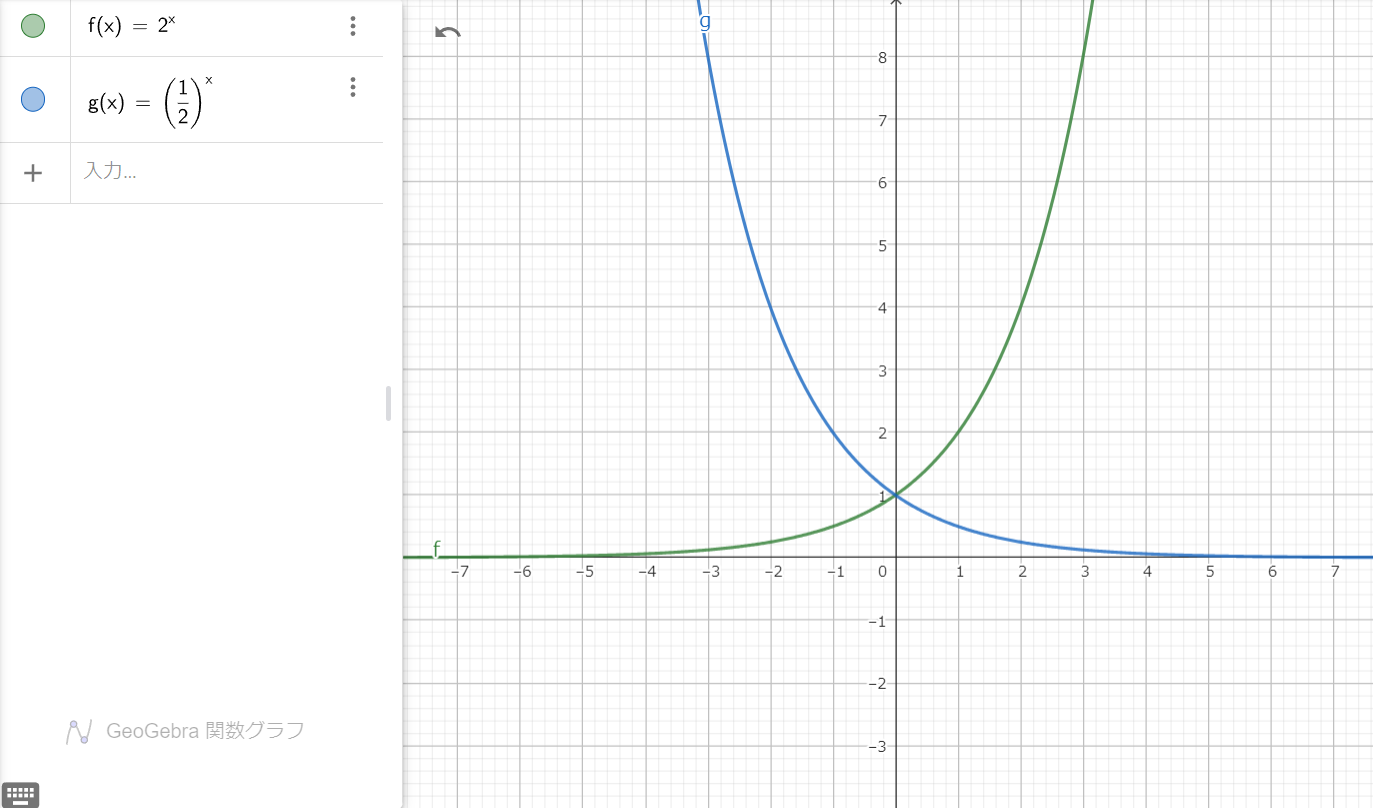
\includegraphics[keepaspectratio,scale=0.3]{img/QuuNote/ExpFuncGraph.png}
                    \caption{指数関数のグラフ}
                \end{figure}

                グラフから、$a$が1より大きくても小さくても$x=0$で$y=1$を取ることがわかる。

                なお、底が$e$の場合の指数関数は$e^x=\exp{x}$と書くこともある。\\

                では次に、指数関数の逆関数を考えてみよう。指数関数の逆関数は与えられた値に対して、
                底を何回掛けたらその値になるかの回数を表す関数である。つまり、指数関数の底ごとに
                逆関数が存在する。文章で見てもわかりずらいので数式で以下示す。

                \begin{equation}
                    f(x)=a^x \leftrightarrow x = f^{-1}(y) = \log_a{y}
                \end{equation}
                指数関数の逆関数は底が何かを示さないといけないので、逆関数$\log$に下付き文字で書く。
                しかし、底が$e$だった場合は省略して$\log y$と書いてもよい。この関数を\textbf{自然対数}という。\footnote{自然対数は$\ln x$と書くこともある。natural logarithmのことである。}
                底が$e$じゃない場合は単に対数と呼ぶ。\footnote{底が10の場合は常用対数という。}

                以下、対数の性質を述べる。必要ない限り底は省略して記載する。指数法則と見比べると理解が深まる。

                \begin{align}
                    \log(xy)&=\log x+\log y\\
                    \log\left(\frac{x}{y}\right)&=\log x - \log y\\
                    \log(a^b) &= b\log a \\
                    \frac{\log_c b}{\log_c a}&=\log_a b\qquad(\text{\textbf{底の変換公式}})
                \end{align}

                また、対数の定義より
                \begin{equation}
                    \log 1 = 0\quad \log_a a = 1
                \end{equation}
                が成り立つ。対数関数$\log x$の引数$x$のことを真数と呼び、これは$x>0$である。\footnote{真数が正であるという条件のことを真数条件という。}

                対数関数のグラフは以下のようになる。

                \begin{figure}[h]
                    \centering
                    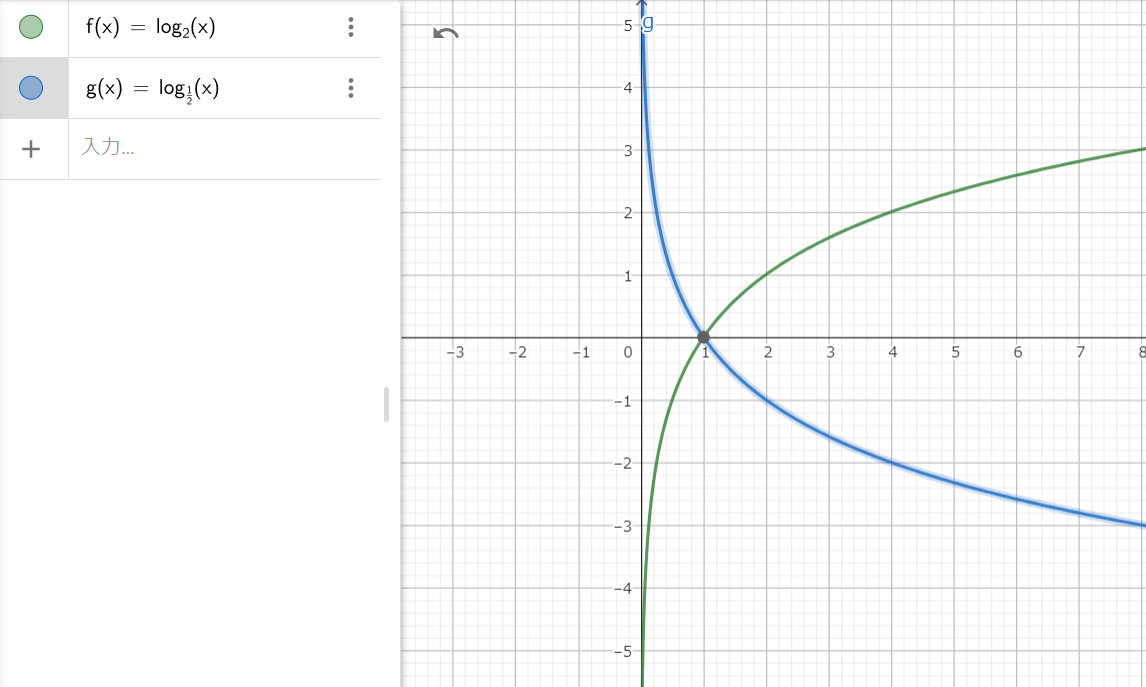
\includegraphics[keepaspectratio,scale=0.5]{img/QuuNote/LogFuncGraph.png}
                    \caption{対数関数}
                \end{figure}
                
                グラフを見ればわかるように、底が1より大きいか小さいかで単調増加・減少かが変わる。

                対数関数は爆発的に増加・減少する指数関数とは対照的に、値の変化が($x<1$を除いて)緩やかである。
                そのため、値がとても大きい値でも対数を取ることで値のスケールを小さくすることができる。
                また、対数を取ることで\underline{掛け算を足し算にできる}。この性質は非常に重要である。
            \clearpage
            \subsection{逆三角関数}
                指数関数の逆関数である対数関数を考えたのと同じように、三角関数の逆関数も考えてみよう。
                三角関数は与えられた角度に対応するそれぞれの三角比を返す関数である。では三角関数の逆関数は
                与えられた三角比に対応する`角度'を返す関数であることがすぐに分かる。これらを次のように書くことにする。
                \begin{align}
                    \arcsin x &= \sin^{-1} x \\
                    \arccos x &= \cos^{-1} x \\
                    \arctan x &= \tan^{-1} x
                \end{align}
                左辺にちなんで左からそれぞれ「アークサイン」,「アークコサイン」,「アークタンジェント」と読む。これらをまとめて
                \textbf{逆三角関数}という。表記に左辺を用いるか右辺を用いるかは個人の好みによる。\footnote{だからといって、$\frac{1}{\sin x}$を$\sin^{-1}x$と書くことはまずない。}

                三角関数が周期関数であるため、逆三角関数は多価関数であることは容易に想像できる。
                逆三角関数を一価関数にするため、値域をそれぞれ$[-\frac{\pi}{2},\frac{\pi}{2}],[0,\pi],[-\frac{\pi}{2},\frac{\pi}{2}]$
                に制限して用いることがある。このことを\ruby{主枝}{しゅし}を取るという。またこの制限した値域を主枝という。
                主枝以外の値域を分枝と呼ぶ。

                逆三角関数が主枝を取っていることを明示するために
                \begin{align}
                    {\rm Arcsin} x &= {\rm Sin^{-1}} x \\
                    {\rm Arccos} x &= {\rm Cos^{-1}} x \\
                    {\rm Arctan} x &= {\rm Tan^{-1}} x
                \end{align}
                のように、先頭を大文字で書くこともある。しかし今回はこの記法は採用しない。

                逆三角関数のグラフは以下のようになる。
                \begin{figure}[h]
                    \begin{minipage}{5cm}
                        \centering
                        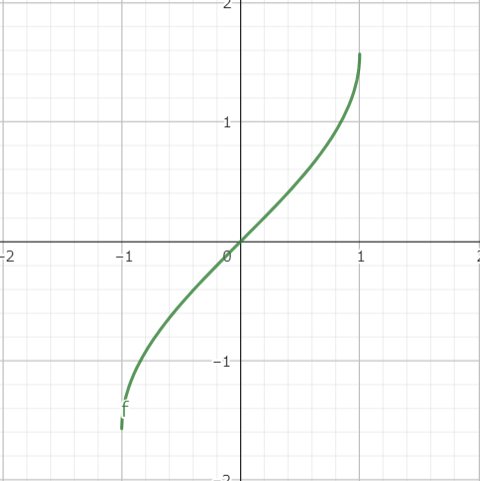
\includegraphics[keepaspectratio,scale=0.3]{img/QuuNote/ArcsinFuncGraph.png}
                        \caption{$\arcsin x$のグラフ}
                    \end{minipage}
                    \begin{minipage}{5cm}
                        \centering
                        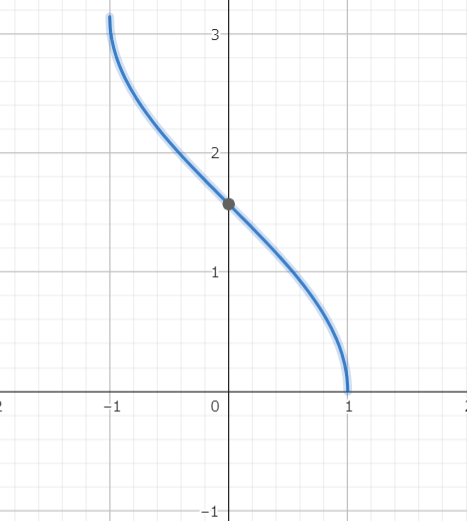
\includegraphics[keepaspectratio,scale=0.3]{img/QuuNote/ArccosFuncGraph_ver2.png}
                        \caption{$\arccos x$のグラフ}
                    \end{minipage}
                    \begin{minipage}{5cm}
                        \centering
                        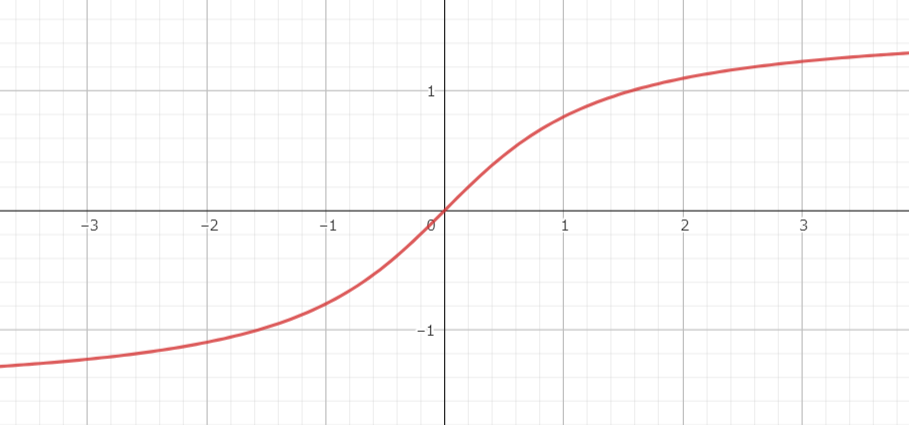
\includegraphics[keepaspectratio,scale=0.3]{img/QuuNote/ArctanFuncGraph.png}
                        \caption{$\arctan x$のグラフ}
                    \end{minipage}
                \end{figure}
                
                もちろん主枝を取らない場合は、それぞれと同じグラフが上や下につながっていく。\\

                三角関数の公式から、逆三角関数についても公式が導ける。例えば、
                \begin{equation}
                    \sin^{-1} x+\cos^{-1} x =\frac{\pi}{2}
                \end{equation}
                ほかにも公式が導けるので、各自で考えてみるとよい。
            \clearpage
            \subsection{双曲線関数}
                いきなりだが、次のように関数を定義する。$e$はネイピア数である。
                \begin{align}
                    \sinh x &= \frac{e^x - e^{-x}}{2}\\
                    \cosh x &= \frac{e^x + e^{-x}}{2}\\
                    \tanh x &= \frac{\sinh x}{\cosh x} = \frac{e^x - e^{-x}}{e^x + e^{-x}}
                \end{align}
                これらは\textbf{双曲線関数}と呼ばれる。読み方はそれぞれ「ハイパボリックサイン」、「ハイパボリックコサイン」、
                「ハイパボリックタンジェント」である。ただこれだと長ったらしいので「シンチ」、「コッシュ」、「タンチ」と呼ぶ
                場合もある。

                見た目が三角関数と酷使しているが、実は性質も似たものを持つ。例えば、$\cosh^2 x - \sinh^2 x = 1$など。
                また、加法定理も符号は若干異なるがほとんど同じ形をしている。

                さらに、オイラーの公式$e^{ix}=\cos x + i\sin x$\footnote{この公式自体はだいぶ後になって解説する。}を用いれば、
                $\sin ix = i\sinh x,\cos ix=\cosh x$が導ける。\footnote{むしろこの性質が成り立つように双曲線関数を定義するといったほうが正しいかもしれない。}\\

                双曲線関数のグラフは以下のようになる。
                \begin{figure}[h]
                    \begin{minipage}{5cm}
                        \centering
                        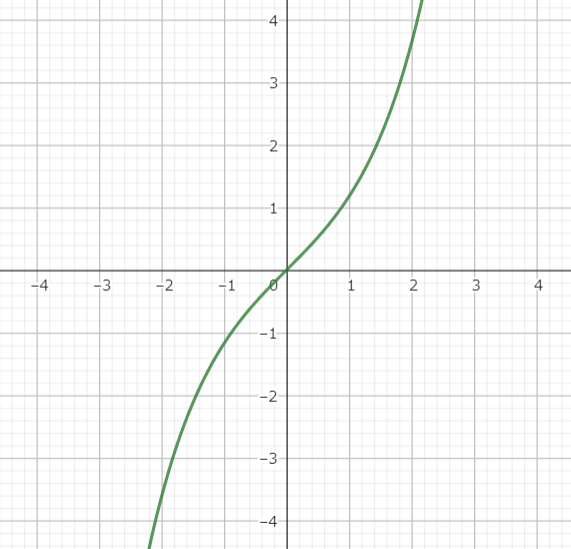
\includegraphics[keepaspectratio,scale=0.3]{img/QuuNote/SinhFuncGraph.png}
                        \caption{$\sinh x$のグラフ}
                    \end{minipage}
                    \begin{minipage}{5cm}
                        \centering
                        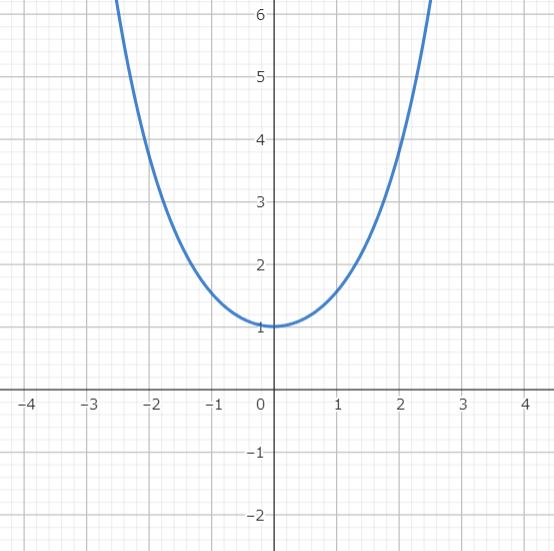
\includegraphics[keepaspectratio,scale=0.3]{img/QuuNote/CoshFuncGraph.png}
                        \caption{$\cosh x$のグラフ}
                    \end{minipage}
                    \begin{minipage}{5cm}
                        \centering
                        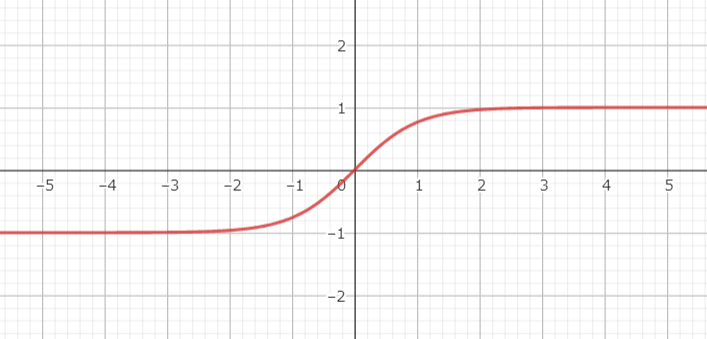
\includegraphics[keepaspectratio,scale=0.3]{img/QuuNote/TanhFuncGraph.png}
                        \caption{$\tanh x$のグラフ}
                    \end{minipage}
                \end{figure}

                $\cosh x$のグラフはカテナリーと呼ばれる。電柱などの垂れた線はこれにあたる。
            \clearpage
            \subsection{初等関数}
                前節まで述べたべき関数、三角関数、指数・対数関数、逆三角関数は\textbf{初等関数}という。
                また、それらの関数からなる多項式の関数や初等関数の合成関数は初等関数である。例えば、双曲線関数は
                $e^x,e^{-x}$の和でなっているが、これらは初等関数なので双曲線関数も初等関数である。

                しかし初等関数の逆関数は必ずしも初等関数であるとは言えない。よく例に挙げられるのが$f(x)=xe^x$の逆関数である。
                この関数はランベルトのW関数とよばれ、$f^{-1}(x)=W(x)$と書かれる。

                初等関数は性質がよく知られているので、微分・積分するうえで比較的扱いやすい。初等関数を微分したもの
                も初等関数であるが、初等関数を積分したものが必ずしも初等関数である保証はない。とはいえ今は微分も積分も知らないわけだから、
                単に事実として受け入れるだけでよい。\\

                初等関数に対して高等関数というものもある。これは初等関数以外の関数のことで、初等関数よりも数は多い。
                先ほど紹介したランベルトのW関数以外には以下のようなものがある。

                \begin{align}
                    \Gamma(s) &= \int_0^\infty e^{-x}x^{s-1}dx\qquad&&(\text{\textbf{ガンマ関数}})\\ 
                    B(p,q) &= \int_{0}^{1} x^{p-1}(1-x)^{q-1}dx\qquad&&(\text{\textbf{ベータ関数}})\\
                    {\rm Li}(x) &= \int \frac{dx}{\log x}\qquad&&(\text{\textbf{対数積分}})\\
                    \zeta(s) &=  \sum_{n=1}^{\infty}\frac{1}{n^s}\qquad&&(\text{\textbf{ゼータ関数}})
                \end{align}

                もちろんこれ以外にも様々な関数がある。興味があったら調べてみるといい。
                \clearpage
                \basicquestion 以下の問いに答えよ。

                \paragraph{問1}次の関数が偶関数か奇関数かを判別せよ。

                \noindent
                (1)$x\sin x$\hspace{3mm}
                (2)$x^5$\hspace{3mm}
                (3)$\sinh x$\hspace{3mm}
                (4)$\log|x^2|$\hspace{3mm}
                (5)$x^3+x+\sin x$\hspace{3mm}
                (6)$e^{-x}$\hspace{3mm}
                (7)$f(\cos x)$\hspace{3mm}
                (8)$\arctan x$

                \paragraph{問2}以下の等式を証明せよ。

                \noindent
                $(1)\sin 2x=2\sin x\cos x/\cos 2x=\cos^2 x-\sin^2 x$(\textbf{倍角の公式})\\
                $(2)\displaystyle \sin^2\frac{x}{2}=\frac{1-\cos x}{2}/\cos^2\frac{x}{2}=\frac{1+\cos x}{2}$(\textbf{半角の公式})\\
                $(3)\sinh(x+y)=\sinh x\cosh y + \cosh x\sinh y/\cosh(x+y)=\cosh(x+y)=\cosh x\cosh y + \sinh x\sinh y$\\
                
                \paragraph{問3}以下の値を求めよ。

                \noindent
                $(1)\sin \pi+\cos \frac{3}{2}\pi + \tan(-\pi)$\hspace{3mm}
                $(2)\arcsin(\frac{1}{2})$\hspace{3mm}
                $(3)\arccos(1)$\hspace{3mm}
                $(4)\log_28$\hspace{3mm}
                $(5)\log_a(\tan(\frac{\pi}{4}))\quad(a>1)$\\
                $(6)\log_63+\log_62$\hspace{3mm}
                $(7)\arcsin(1-\log\pi)-\cos(\log2)\sin(\log 3)+\sin(\log3 -\log 2)-\log e^{\arccos(\log \pi-1)}$

                \paragraph{問4}対数を使えば桁数の多い数字同士の掛け算を足し算で計算することができる。簡単な例として$271\times 314$を
                対数を用いて計算せよ。ただし、常用対数$\log_{10} 2.71\simeq0.4346,\log_{10} 3.14\simeq0.4969,10^{4.9315}\simeq85408$は用いてよい。
                
                \paragraph{問5}$t=\tan\frac{x}{2}$とするとき、$\sin x,\cos x,\tan x$をそれぞれ$t$を用いた式で表せ。\footnote{ヒント:半角の公式を用いる。}
            \clearpage
            \section{極限}
            \subsection{数列の極限}
                \textbf{数列}とは、数字をある規則によって並べた列のことで、例えば$1,2,3,4,\cdots,100$などがある。
                この数字に左から順に番号付けすることを考える。そのときある数列$\{a_n\}$について、左から$n$番目の数値を$a_n$
                と表し、第$n$項とよぶ。特に$n=1$の一番初めの項$a_1$を初項という。
                数列には等差数列や階差数列があるがここでは詳しく述べない。

                項の数は有限でも無限でもよいので、項が無限にある数列$\{a_n\}$について考えてみることにする。$n$を限りなく大きくすると
                数列の値がある一定の値$a$に近づくときがある。この時数列$\{a_n\}$は\textbf{収束する}といい、近づく値$a$を\textbf{極限値}
                という。これを数式で表すと
                \begin{equation}
                    \lim_{n\to \infty}a_n=a
                \end{equation}
                新しく$\lim$という記号が出てきたが、これは$n$を限りなく大きくする(無限大に近づける)という操作を表す記号である。
                $a_n\to a \hspace{1mm}(n\to\infty)$と書いてもよい。このとき$a_n=a$となる$n$が存在する必要はない。
                
                \paragraph*{例}$\{a_n\}=1-\frac{1}{n}$について考える。$n$を限りなく大きくすると$\frac{1}{n}$は限りなく小さくなる($0$に近づく)ので
                $a_n$は$1-0=1$に近づく。よって$\{a_n\}$は収束し、極限値は$1$。\\

                始めのうちは値が近づく、と言われても何をどうすればよいかわからないであろうから、代入のような何かという風にとらえてもよい。実際極限のほとんどの操作は
                代入と結果的に等しくなる。気を付けないといけないは代入だと定義できない$\frac{1}{0}$などの場合である。\\

                極限の性質について以下にまとめる。$\displaystyle\lim_{n\to\infty}a_n=a,\lim_{n\to\infty}b_n=b,cは定数$とする。
                \begin{align}
                    \lim_{n\to\infty}(a_n\pm b_n)&=a\pm b\\
                    \lim_{n\to\infty}(c\cdot a_n)&=c\cdot a\\
                    \lim_{n\to\infty}(a_n\cdot b_n)&=a\cdot b\\
                    \lim_{n\to\infty}\frac{a_n}{b_n}&=\frac{a}{b}\quad(b_n\neq 0,b\neq 0)
                \end{align}

                収束するとは$n$を限りなく大きくしたときに数列が有限の値に近づくことだが、これはより厳密に言うことができる。
                \begin{itembox}{数列の収束の定義}
                    数列$\{a_n\}$が$a$に収束する$\Leftrightarrow $任意の$\varepsilon>0$が与えられたとき、それに対応してある$N$が\fbox{$n>N$のとき$|a-a_n|<\varepsilon$}となるように定められる。
                \end{itembox}
                正直一目見ただけでは全然意味がわからないはず。少しずつ理解していこう。この定義は二つに分けると見やすい。
                まず、任意の$\varepsilon$、つまりどんな$\varepsilon>0$に対しても、(収束するなら)対応する$N$が必ず見つかるということを言っている。
                ただ、このままだとなにをどう対応する$N$なのかがはっきりしない。そこで四角で囲った条件が必要になる。ざっくり言ってしまえば
                \underbar{正数$\varepsilon$がどんな値でも、四角で囲った条件を満たす$N$が見つかる}ということになる。

                次に四角で囲った条件について詳しく見ていこう。始めの条件$n>N$は一旦無視して、$|a-a_n|<\varepsilon$に注目する。
                この不等式の左辺が何を表すかを考えてみよう。数直線上に$a,a_n$をプロットすると、$|a-a_n|$はそのプロットした点と点
                との距離を表す。つまり不等式は、「近づく(であろう)値と$a_n$との距離をどんなに小さくとっても\footnote{$\varepsilon$は任意の数なのでどんなに小さくとってもよい。
                反対に大きくとることもできるが、$<\varepsilon$なので大きくとることに言及する意味はない。}」という意味になる。
                ここで飛ばした$n>N$についてみてみると、これは$n$が$\varepsilon$によって決まる$N$より大きい、という意味であるから、
                四角の条件をまとめると「近づく(であろう)値と$a_n$との距離をどんなに小さくとっても、その小さくとった幅に対応して$n$を大きくとれる」ということになる。\\

                とはいえ、これを文章で説明されても全然イメージがわかない。ということで実際に値をプロットしてみた。
                \begin{figure}[h]
                    \centering
                    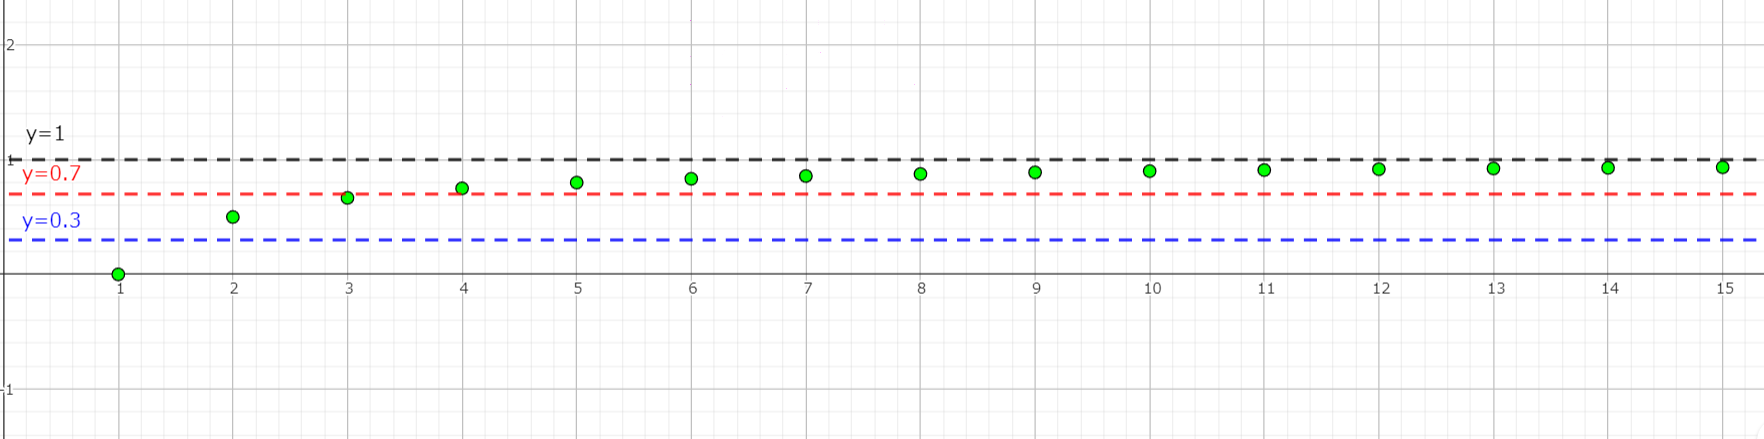
\includegraphics[keepaspectratio,scale=0.45]{img/QuuNote/SequeanceLimitGraph.png}
                    \caption{$\{a_n\}=1-\frac{1}{n}$のグラフ}
                \end{figure}
                
                この数列で「$\varepsilon=0.7$を取るとき、$|a-a_n|=\frac{1}{n}<0.7\to n> 1=N$となるように$N$を取れば、$n>N$となる全ての$a_n$は
                図中の黒線と青線の間に入っている」が成り立っている。
                次の「$\varepsilon=0.3$を取るとき、$|a-a_n|=\frac{1}{n}<0.3\to n>3=N$となるように$N$を取れば、$n>N$となる全ての$a_n$は
                図中の黒線と青線の間に入っている」も成り立っている。

                このように「黒線との距離がどんなに小さな点線を考えても、ある番号$N$以上なら黒線とその小さい点線の間にプロットされる。そのような$N$が必ず見つかる。」というのが収束の定義の主張である。\\

                この収束の定義はとても難しい話なので、理解するのに時間がかかるかもしれない。(丁寧に説明したつもりけど、逆に回りくどくなってわかりにくいかも)そんな時は一旦飛ばすというのも手である。
                もちろんここで立ち止まって考えてもいいが一旦放置してあとから見直すとわかる、なんてこともざらにある。\\

                {\color{blue}$\diamondsuit$収束する数列はすべて有界\footnote{有界とは全ての$n$に対して$m\leq a_n \leq M$である定数$m,M$が存在すること。}である。\footnote{詳しい話は無限級数を扱うときに述べる。}}
            \clearpage
            \subsection{関数の極限}
                次の関数の極限について述べる。数列と違い、無限大以外に近づける場合も出てくる。ひとまず定義域$x\in I=(a,b)$である関数$f(x)$と
                定数$c\in I$を考えよう。$x$の値を$c$に限りなく近づけたとき、$f(x)$の値がある一定の値$C$に近づくとする。
                このとき
                \begin{equation}
                    \lim_{x\to c}f(x)=C
                \end{equation}
                と表し、$f(x)$は\textbf{収束する}という。また、$C$を$x$を$c$に近づけたときの$f(x)$の\textbf{極限値}という。記号の使い方は数列と同じなので馴染みやすい。
                もちろん$f(x)\to C\quad(x\to c)$という書き方もできる。
                
                \paragraph{例}$\displaystyle\lim_{x\to 2}x^2 = 4$ $x<2$の点からでも$x>2$の点からでも$2$に近づければ$f(x)=4$に近づく。これはグラフを見ても直感的にわかる。\\
                
                いま$c$は$f(x)$の定義域に含まれている状態で考えてみるが、実は含まれていなくてもよい。
                例えば、$f(x)=\frac{x^2-1}{x-1}$は$x=1$で定義出来ないが、$x\neq 1$で$f(x)=x+1$であるから$x\to 1$の
                極限を取ると値は$2$に近づく。このような例で極限と代入との違いがはっきりとわかる。\\

                いま近づけている値は有限の値を想定しているが、数列のように無限大(小)に大きくする極限も考えることが考えることができる。
                \begin{equation}
                    \lim_{x\to\infty}f(x)\quad \lim_{x\to-\infty}f(x)
                \end{equation}
                のように書く。例えば、$\displaystyle\lim_{x\to \pm\infty}\frac{1}{x}=0$。
                
                \noindent
                極限の性質の公式は、数列と同様であるためここでは述べない。\\

                さて、数列の極限と同様、関数の極限でもより厳密な定義について考えてみよう。それは以下のようになる。
                \begin{itembox}{関数の極限の定義}
                    $f(x)$が$x\to a$で$b$に収束する$\Leftrightarrow$任意の$\varepsilon>0$が与えられたとき、それに対応してある$\delta > 0$が\fbox{$|x-a|<\delta$のとき$|f(x)-b|<\varepsilon$}
                    となるように定められる。
                \end{itembox}
                これはいわゆる\textbf{$\varepsilon-\delta$論法}と呼ばれるもので、ぶっちゃけめっちゃ難しい。ただこれも落ち着いてみれば数列の極限の定義\footnote{$\varepsilon-N$論法という。}と似通っているところがあることに気づける。

                数列の極限との違いは$x$の範囲の制限にある。数列の場合は$x>N$だったが、関数の場合は$|x-a|<\delta$となっている。$N,\delta$の役割は同じなので今はただ記号を変えているだけと考えてよい。
                $|x-a|$は$x$と$a$との数直線上での差、つまり二つの点の距離を表しているので、$|x-a|<\delta$はその距離が$\delta$より小さいときというのを表している。
                あとは数列の場合と大体同じで、どんなに$f$と極限値が近づいていても($\varepsilon$を小さくしても)それに対応する$\delta$の値が定められる($x$が$a$に近づく)ということになる。
                \newpage

                $\varepsilon-\delta$論法を使って、実際に収束することを証明してみる。
                \paragraph*{例}$\displaystyle\lim_{x\to 2}x^2=4$を証明する。\\
                $|x-2|<\delta$とするとき、$|x^2-4|=|x-2|\cdot|x+2|=|x-2|\cdot|(x-2)+4|\leq |x-2|^2+4|x-2|<\delta^2+4\delta$
                であるため、$\varepsilon=\delta^2+4\delta\leftrightarrow \delta = -2+\sqrt{4+\varepsilon}$となるように$\delta$を取ればよい。このとき$|x-2|<\delta\rightarrow|x^2-4|<\varepsilon$を満たすので証明が終わる。$\square$\\

                試しに、$\varepsilon = 0.1$を代入すると$\delta \thickapprox 0.02484$であるため、$x=2.02483$のとき$|x^2-4|<\varepsilon$を満たすはずである。
                実際、$|x^2-4|=0.0999770256<0.1=\varepsilon$となっていて満たしている。今回は具体的に$\delta(\varepsilon)$を求めたが、このやり方にとらわれなくても四角で囲った条件を満たすように$\delta$が
                取れればよい。\\

                ここまで関数の収束について述べたが、ある一定の値に近づかずそのまま値が無限大に増大する場合などについて考えてみる。
                例えば、$x^3$は$x\to\infty$で$x^3\to\infty$である。このような場合\textbf{無限大に発散する}という。
                もちろん負の無限大に発散する場合も考えられる。一方で、$\sin x$は$x\to\infty$で値が無限大に増大するわけではないが、
                値が一つに定まることもない。このような場合は\textbf{振動する}という。\footnote{$\sin x$のグラフを見れば「振動する」という言い方がぴったりだとわかる。}\\

                次に重要な極限の公式を述べる。
                \begin{align}
                    \lim_{x\to 0}&\frac{\sin x}{x}=1\label{eq:limit of sin/x}\\
                    \lim_{x\to 0}&\left(1+x\right)^\frac{1}{x} = e\label{eq:define_e}
                \end{align}
                式(\ref{eq:define_e})はネイピア数の定義である。実際は左辺の極限が収束することを証明しないといけないが、ここでは割愛する。

                では式(\ref{eq:limit of sin/x})を証明する。
                \paragraph{証明}下図のような単位円を考える。
                \begin{figure}[h]
                    \centering
                    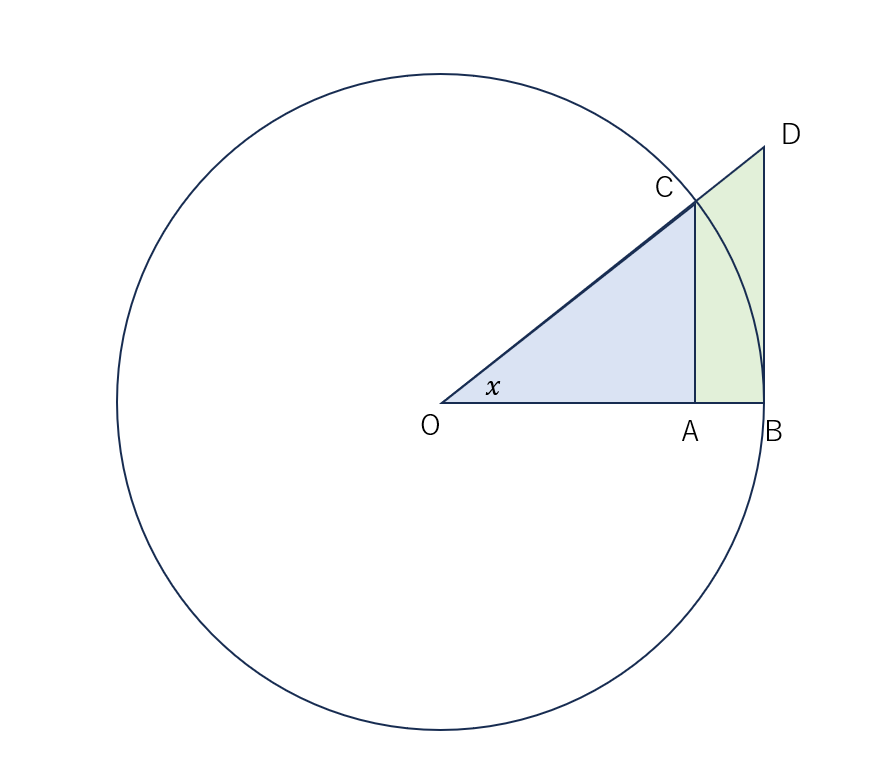
\includegraphics[keepaspectratio,scale=0.3]{img/QuuNote/circleFor_sin_div_xLimit.png}
                    \caption{単位円}
                \end{figure}

                このとき$\triangle OAC< OBC < \triangle OBD$である。それぞれ$\frac{1}{2}OA\cdot AC,\frac{1}{2}OC^2x,\frac{1}{2}OB\cdot BD$なので
                
                \begin{alignat}{3}
                    \frac{1}{2}OA\cdot AC&<& \frac{1}{2}OC^2x &<& \frac{1}{2}OB\cdot BD\notag\\
                    \frac{1}{2}OC^2 \sin x\cos x & < & \frac{1}{2}OC^2 x & < & \frac{1}{2}OC^2\tan x\notag\\
                    \sin x\cos x & < & x & < & \tan x\notag\\
                    \cos x & < & \frac{x}{\sin x} & < & \frac{1}{\cos x}\notag\\
                    \cos x & < & \frac{\sin x}{x} & < & \frac{1}{\cos x}\label{eq:Hasamiuti}
                \end{alignat}
                よって、$x\to 0$の極限を取れば$\displaystyle \cos x\to 1,\frac{1}{\cos x}\to 1$より$\displaystyle\frac{\sin x}{x}\to 1$となる。$\square$\\

                最後の不等式(\ref{eq:Hasamiuti})のような不等式のとき、両側の極限値が一致すれば、間に挟まれた極限値も等しくなる。これを\textbf{はさみうちの原理}という。
                はさみうちの原理ではうまく挟み込める不等式をつくる必要があるので、慣れるまで時間がかかる。

            \clearpage
            \subsection{極限の計算}
                この節では実際に極限の計算方法について学ぶ。単純な場合は代入と同様に計算してよいが$\frac{0}{0}$などの形になる場合は式を変形する必要がある。

                \paragraph{例1}次の極限を求めよ。
                    \begin{equation*}
                        \lim_{x\to \infty}\frac{x^3+5x^2+x+2}{x^3+x+10}
                    \end{equation*}
                    $\frac{1}{x}\to 0(x\to \infty)$の結果を利用する。分子と分母に$\frac{1}{x^3}$をかけて
                    \begin{equation*}
                        \lim_{x\to \infty}\frac{1+\frac{5}{x}+\frac{1}{x^2}+\frac{2}{x^3}}{1+\frac{1}{x^2}+\frac{10}{x^3}}=\frac{1+0+0+0}{1+0+0}=1
                    \end{equation*}
                
                \paragraph{例2}次の極限を求めよ。
                    \begin{equation*}
                        \lim_{x\to 0}\frac{x}{1-\sqrt{x+1}}
                    \end{equation*}
                    $(a-b)(a+b)=a^2-b^2$を用いる。分子と分母に$1+\sqrt{x+1}$をかけて
                    \begin{equation*}
                        \lim_{x\to 0}\frac{x(1+\sqrt{x+1})}{(1-\sqrt{x+1})(1+\sqrt{x+1})}=\lim_{x\to 0}\frac{x(1+\sqrt{x+1})}{-x}=-(1+\sqrt{0+1})=-2
                    \end{equation*}
                
                \paragraph{例3}次の極限を求めよ。
                    \begin{equation*}
                        \lim_{x\to\infty}\frac{2^x+1}{3^x}
                    \end{equation*}
                    $x$が十分大きいとき$2^x\ll 3^x$であるため、直感的に極限値は0だとわかる。
                    \begin{equation*}
                        \lim_{x\to\infty}\left(\left(\frac{2}{3}\right)^x+\frac{1}{3^x}\right)=\lim_{x\to\infty}\left(\frac{2}{3}\right)^x+\lim_{x\to\infty}\frac{1}{3^x}=0+0=0
                    \end{equation*}
                    二項目は指数関数の性質$a^x\quad(a<1)$の場合を用いた。三項目は$x\to\infty$のとき$3^x\to\infty$であることを用いた。

                \paragraph{例4}次の等式を証明せよ。
                    \begin{equation*}
                        \lim_{x\to \infty}\left(1+\frac{1}{x}\right)^x = \lim_{x\to 0}\left(1+x\right)^\frac{1}{x} 
                    \end{equation*}
                    $x=\frac{1}{t}$と置くと、$x\to\infty$で$t\to0$だから
                    \begin{equation*}
                        \lim_{x\to \infty}\left(1+\frac{1}{x}\right)^x = \lim_{t\to 0}\left(1+\frac{1}{\frac{1}{t}}\right)^\frac{1}{t}=\lim_{t\to\infty}(1+t)^\frac{1}{t}
                    \end{equation*}
                    よって等式が成り立つ。\\

                もちろんこれ以外にも極限の計算を行う際に用いるテクニックは存在するが、もう少し勉強を進めないと使うことができない。その時が来るまで楽しみにしていてほしい。
                なお、これらのテクニックのほとんどは数列の極限にも用いることができる。
            \clearpage
            \subsection{関数の連続}
                次に、関数の連続について考えていく。ひとまず定義から述べる。関数$f(x)$が$x=a$で\textbf{連続}であるとは、次の三つの条件を満たすことである。
                \begin{enumerate}
                    \item $f(a)$が定義されている。
                    \item $\displaystyle\lim_{x\to a}f(x)$が存在する。
                    \item $\displaystyle f(a)=\lim_{x\to a}f(x)$である。
                \end{enumerate}
                極限の場合は$x=a$で値が存在していなくてもよかったが、連続では$x=a$での値も必要となる。

                連続の条件2について、極限が存在するとはどういうことなのか考えてみよう。関数の極限$x\to a$では、\underline{$x$をどのように$a$
                に近づけても同じ極限値を取る}必要がある。
                どのように近づけても、と言われて困るかもしれないが、単に$x>a$の点と$x<a$の点から近づける場合を考えておけばよい。\footnote{二変数関数になると少し事情は変わる。`xy平面上のどの点から'近づけても同じになる必要がある。}

                このうち、$x>a$の点から近づける場合、すなわち数直線の右側から近づける場合を$\displaystyle\lim_{x\to a+0}f(x)$と表し、\textbf{右側極限値}と呼ぶ。
                同様に$x<a$の点から近づける場合は$\displaystyle\lim_{x\to a-0}f(x)$と表し、\textbf{左側極限値}と呼ぶ。この右側極限値と左側極限値が等しくなる時、
                極限は存在し、その値は
                \begin{equation}
                    \lim_{x\to a}f(x)=\lim_{x\to a+0}f(x)=\lim_{x\to a-0}f(x)
                \end{equation}
                となる。

                関数$f(x)$がある区間$I$で連続であるとき、$f(x)$は$I$で\textbf{連続関数}であるという。例えば、$f(x)=\sin x$は区間$(-\infty,\infty)$で連続関数である。
                一般に、初等関数は値が定義される(無限大にならないなど)全ての$x$について連続である。

                関数がある区間で連続であるといったが、そもそも区間の端での連続はどう定義すればよいだろうか。
                例えば、関数$f(x)=\sqrt{x}$は明らかに$x\geq 0$のすべての$x$で定義されているが$x=0$において連続の条件
                が適用できない。そこで、一般に関数が$x\geq a$で定義されているとき
                \begin{equation}
                    \lim_{x\to a+0}f(x)=f(a)
                \end{equation}
                が成り立てば、$x=a$において連続であるとする。こう定義することで、$\sqrt{x}$が区間$x\geq 0$で連続と定義できる。
                同様にして$x\leq b$である場合の端でも連続が定義される。この場合
                \begin{equation}
                    \lim_{x\to b-0}f(x)=f(b)
                \end{equation}
                のように左極限を取ることに注意。\\

                以下連続関数の性質について述べる。まず連続関数$f(x),g(x)$について
                \begin{equation}
                    f(x)\pm g(x)\quad f(x)g(x)\quad \frac{f(x)}{g(x)}
                \end{equation}
                は連続関数である。ただし、最後の式は$g(x)\neq 0$であるとする。このことから、連続関数の多項式も連続関数であることがわかる。\\

                \noindent
                例えば、$f(x)=x^n(n\in\mathbb{N})$は区間$(-\infty,\infty)$で連続であるため、多項式
                \begin{equation}
                    P(x)=a_nx^n+a_{n-1}x^{n-1}+\cdots+a_{1}x+a_0
                \end{equation}
                も区間$(-\infty,\infty)$で連続である。ほかにも、以下の\textbf{有理関数}
                \begin{equation}
                    R(x)=\frac{a_nx^n+a_{n-1}x^{n-1}+\cdots+a_{1}x+a_0}{b_nx^n+b_{n-1}x^{n-1}+\cdots+b_{1}x+b_0}
                \end{equation}
                も分母が0にならない限り連続である。

                また、次の\textbf{合成関数}$f(g(x))$を考えてみると、$f(x),g(x)$が連続関数であるかぎり$f(g(x))$も連続関数である。
                例えば$\log(\sqrt{x}+1)$は$x\geq 0$のすべての$x$で連続である。\\

                関数$f(x)$が区間$[a,b]$で連続関数である場合、次の二つが成り立つ。
                \begin{screen}
                    $f(a)\neq f(b)$なら$f(a)\leq k \leq f(b)$である任意の$k$について
                    \begin{equation*}
                        f(x)=k
                    \end{equation*}
                    となる点$c\in[a,b]$が少なくとも一つ存在する。(\textbf{中間値の定理})
                \end{screen}
                \begin{screen}
                    $f(x)$は区間$[a,b]$で必ず最大値$M$と最小値$m$を取る。つまり
                    \begin{equation*}
                        m=f(x_m)\leq f(x)\leq f(x_M)=M
                    \end{equation*}
                    となる点$x_m,x_M\in[a,b]$が必ず存在する。
                \end{screen}
                文字だけだとわかりずらいが、グラフを見ればむしろ当たり前のことのように感じる。
                \begin{figure}[h]
                    \centering
                    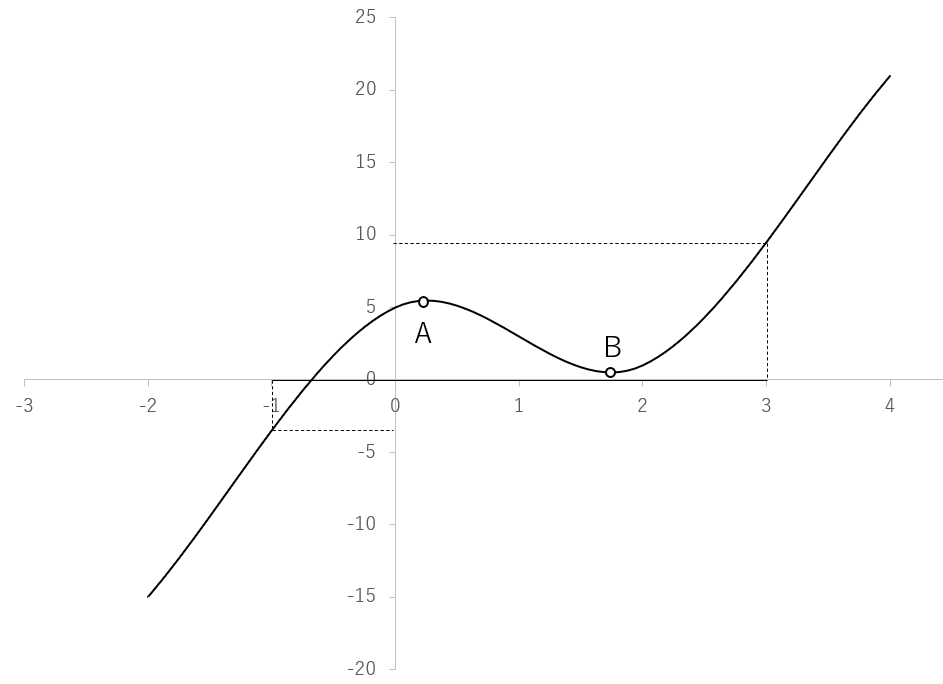
\includegraphics[keepaspectratio,scale=0.3]{img/QuuNote/ContinuousFuncGraph.png}
                    \caption{連続関数}\label{fig:連続関数,中間値の定理,最大最小}
                \end{figure}

                図\ref{fig:連続関数,中間値の定理,最大最小}を見ると、区間$[1,3]$において関数は連続であり、その端での値
                おおよそ$-3$と$9$の間のすべて値に対して、対応する$x\in[-1,3]$が存在していることがわかる。これが中間値の定理
                の主張である。また区間における最大値と最小値も存在している(それぞれ$x=-1,3$の点)ことがわかる。
                ちなみに、点A,Bはそれぞれその周囲の点の間では最大・最小の値である。これらをそれぞれ極大値、極小値とよび、総称して
                \textbf{極値}という。
                \newpage
                また、中間値の定理において$f(a)$と$f(b)$の符号が異なる場合、方程式$f(x)=0$は
                区間$[a,b]$に実数解を少なくとも持つことがわかる。これは中間値の定理の応用である。
                \paragraph{例}方程式$x^2+x+1=0$は区間$[-1,1]$に少なくとも一つの実数解を持つかどうか答えよ。

                $f(-1)=1-1+1=1>0,f(1)=1+1+1=3>0$より、$f(-1)$と$f(1)$の符号が同じであるため方程式は区間$[-1,1]$で実数解を持たない。
                実際、判別式$D=1^2-4\cdot 1\cdot 1=-3<0$より、この二次方程式は解を持っていない。\\

                いままでは連続関数の性質について述べたが、連続の条件が一つでも満たされていない場合についても考えてみよう。
                このとき関数$f(x)$は$x=a$で\textbf{不連続}であるという。例えば$\frac{1}{x}$は$x=0$で不連続である。
                一方で関数$\displaystyle g(x)=\frac{x^2-1}{x-1}$も$x=1$で不連続であるが、$x\neq1$では$g(x)=x+1$で連続である。
                そこで、
                \begin{equation}
                    g(x)=\left\{\begin{array}{lr}\displaystyle\frac{x^2-1}{x-1}&(x\neq 1)\\\displaystyle x+1&(x=1)\end{array}\right.
                \end{equation}
                のように改めて定義しなおすことで、この関数は$x=1$で連続にできる。各自確かめてみよ。
            \clearpage
            \basicquestion 以下の問いに答えよ。

                \paragraph{問1}以下の数列の一般項を示し、それらが収束するかどうか答えよ。\\
                $(1)\{a_n\}=\frac{2}{1},\frac{3}{2},\frac{4}{3}\cdots$\hspace{3mm}
                $(2)\{b_n\}=\frac{1}{3},\frac{1}{9},\frac{1}{27}\cdots$\hspace{3mm}
                $(3)\{c_n\}=1,-1,1,-1\cdots$\\
                $(4)\{d_n\}=a,a+d,a+2d,a+3d\cdots(a,dは定数)$

                \paragraph{問2}以下を証明せよ。
                \begin{equation*}
                    \lim_{n\to\infty}(a_n+b_n)=a+b
                \end{equation*}
                ただし、$\displaystyle\lim_{n\to\infty}a_n=a,\lim_{n\to\infty}b_n=b$とする。{\scriptsize ヒント:$\varepsilon-N$論法を用いる。}

                \paragraph{問3}以下計算せよ。\\

                \noindent
                $(1)\displaystyle \lim_{x\to 0}\frac{\sin2x}{x}$\hspace{3mm}
                $(2)\displaystyle \lim_{x\to 2\pi}\sin \frac{x}{2}+x^2$\hspace{3mm}
                $(3)\displaystyle \lim_{x\to\infty}\frac{x^2+x+1}{x^3+1}$\hspace{3mm}
                $(4)\displaystyle \lim_{x\to 0}\frac{x^2}{1-\cos x}$\hspace{3mm}
                $(5)\displaystyle \lim_{x\to 0}\tan x$\hspace{3mm}
                $(6)\displaystyle \lim_{x\to\infty}\frac{2^x+3^x}{2^x-3^x}$\\
                $(7)\displaystyle \lim_{x\to 0}\frac{\sqrt[3]{8+x}-2}{x}$\hspace{3mm}
                $(8)\displaystyle \lim_{x\to 0}\frac{e^x-1}{x}$
                
                \paragraph{問4}次の関数が()内の点において連続であるかどうか調べよ。\\
                $(1)f(x)=x^2\quad(x=2)$\hspace{1mm}
                $(2)f(x)=\sin x\quad(x=\frac{\pi}{2})$\hspace{1mm}
                $(3)f(x)=\sqrt{1-x^2}\quad(x=1)$\hspace{1mm}
                $(4)f(x)=\frac{1}{\sqrt{x}}\quad(x=0)$\\
                $(5)f(x)=|x|\quad(x=0)$\hspace{1mm}
                $(6)\displaystyle f(x)=\left\{\begin{array}{lr}\displaystyle x\sin\frac{1}{x}&(x\neq 0)\\1&(x=0)\end{array}\right.$\\

                \paragraph{問5}方程式$\sin x=x$が区間$[0,\frac{\pi}{2}]$に実数解をもつかどうか調べよ。
            \clearpage
            \section{第I部演習問題}
                \paragraph{問1} 以下の計算をせよ。ただし$(2)$において$-1<x<1$とする。
                    \begin{alignat*}{9}
                        &[1]\log\sqrt{2+\sqrt{3}} &[2]&\sin^{-1}x+\cos^{-1}x &[3]&\cos\left(\frac{5\pi}{12}\right) & [4]&\log(e^{x^2}) & [5]&\sin(12\pi)\\
                        &[6]\lim_{x\to 0}x^n(n\in\mathbb{N}) &[7]&\lim_{n\to 0}x^n &[8]&\lim_{n\to 0}(\sqrt{n^2+3n}-n) &[9]&\lim_{n\to\infty}(\sqrt[3]{n+1}-\sqrt[3]{n}) & [10]&\lim_{x\to +0}x^x\\
                        &[11]\lim_{x\to +0}\frac{\sin x}{\sqrt{x}} &[12]& \lim_{x\to\infty}\frac{\sin(x)}{x} &[13]&\lim_{n\to\infty}\sum_{k=1}^{n}k\cdot\left(\frac{k}{n}\right) &[14]&\lim_{t\to 0}\frac{(x+t)^2-x^2}{t}
                    \end{alignat*}
                \paragraph{問2}次の式について以下の問いに答えよ。
                    \begin{equation}
                        \lim_{n\to n}a_n=a \Rightarrow \lim_{n\to\infty}\frac{a_1+a_2+\cdots+a_n}{n}=a
                    \end{equation}
                    \begin{description}
                        \item[(1\textrm{)}] 上式を証明せよ。
                        \item[(2\textrm{)}] $\log\left(\frac{2}{1}\times\frac{3}{2}\times\cdots\times\frac{n+1}{n}\right)-\log\frac{n+1}{n}$を求めよ。
                        \item[(3\textrm{)}] $\displaystyle \lim_{n\to\infty}\frac{\log n}{n}$を求めよ。
                    \end{description}
                
                \paragraph{問3}
                    次の関数が$[\quad]$の点で連続であるかどうか答えよ。
                    \begin{align*}
                        (1)&\sign x = \left\{\begin{array}{cc}\displaystyle 1 & (x>0) \\ 0 & (x=0) \\ -1 & (x<0)\end{array}\right.&\quad [x=0]\\
                        (2)&f(x)=\lim_{n\to \infty}f_n(x)\quad (f_n(x)=x^n\quad(0\leq x\leq 1))&\quad [x=1]
                    \end{align*} 
                    (1)の関数は\textbf{符号関数}という。${\rm sgn}(x)$と書く場合もある。

                \paragraph{問4}
                    数学において$0^0$は$1$と定義されたりそもそも定義されなかったりする。さて、$0^0=1$と定義する立場での根拠について関数$f(x)=x^x$を用いて極限の観点から述べよ。
                
                \linktoMOKUZI
                
    \clearpage
    \part{微分法$f'$}
    \vspace{\stretch{1}}
    \begin{screen}
        いよいよ微分積分の``微分''の話に移る。微分法は、関数の挙動について解析するときに用いる。具体的な計算は公式に当てはめるだけなので
        そこまで難しくない。それにもかかわらず微分の応用例は幅広い。理屈がわかったらあとは練習あるのみである。
        また、この章ではテイラー展開などについても扱う。
    \end{screen}
    \clearpage
    \section{導関数}
        \subsection{平均変化率・微分係数}
            一次関数$y=\alpha x+b$の傾き$\alpha$を求める方法は直線上の二点の座標がわかればよく、それらを$(x_1,y_1),(x_2,y_2)$と置けば、
            \begin{equation}
                \alpha=\frac{y_2-y_1}{x_2-x_1}
            \end{equation}
            で求まる。また分子と分母はそれぞれ$(x_1,y_1)$からの$x$方向$y$方向の変化分だと考えられるので、それらを$\Delta x=x_2-x_1,\Delta y=y_2-y_1$と置けば
            \begin{equation}
                a= \frac{\Delta y}{\Delta x}
            \end{equation}
            となる。これを一般の関数$y=f(x)$に拡張することを考える。ここで注意しておいてほしいのは、
            一般の関数で考える際は$(x_1,y_1),(x_2,y_2)$の取り方によって傾きの値が変わってしまうことである。

            例えば、$y=x^2$について$(1,1^2)$から$(2,2^2)$の傾きは$\frac{4-1}{2-1}=3$だが、
            $(3,3^2)$から$(4,4^2)$の傾きは$\frac{16-9}{4-3}=7$となってしまう。つまり$x$の増分が同じであっても
            $y$の増分が同じであるとは限らないのである。

            とはいえ、傾きの式を$y=f(x)$の場合で拡張するからなにか定義の式が変わるわけではない。やはり二点の座標について
            \begin{equation}
                \frac{f(x_2)-f(x_1)}{x_2-x_1}\quad\left(=\frac{y_2-y_1}{x_2-x_1}\right)
            \end{equation}
            となる。この$x$の増分と$y$の増分の比のことを\textbf{平均変化率}という。
            \begin{figure}[h]
                \centering
                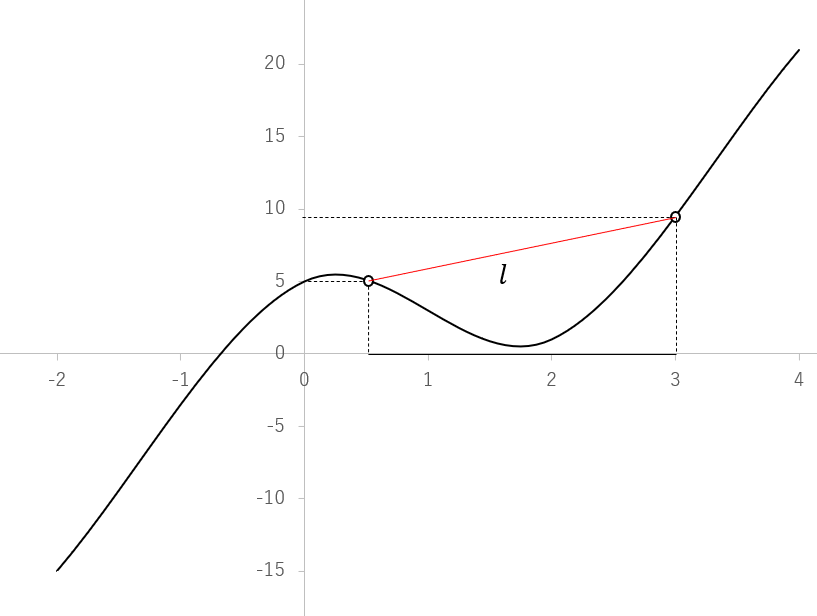
\includegraphics[scale=0.3]{img/QuuNote/heikinhenkaritu.png}
                \caption{平均変化率と直線}
            \end{figure}

            上図のように、平均変化率は二点を結んだ直線$l$の傾きを表している。また$a=x_1,b=x_2$と置き、$a$と$b$の差を$h=b-a$と置けば、
            \begin{equation}
                \frac{f(a+h)-f(a)}{h}
            \end{equation}
            と表すこともできる。
            
            次に点$x=b$を点$x=a$に限りなく近づける場合を考えよう。これは$a$と$b$との距離が限りなく小さくなることを意味するので$h\to 0$の極限である。すなわち
            \begin{equation}
                \lim_{h\to 0}\frac{f(a+h)-f(a)}{h}
            \end{equation}
            となる。この極限値が存在する場合、$f(x)$は$x=a$で\textbf{微分可能}であるという。また、その値を$x=a$における$f(x)$の\textbf{微分係数}といい、$f'(a)$と表す。
            \clearpage
            $h$は右側(正の側)から0に近づく場合と左側(負の側)から0に近づく場合がある。
            前者を\textbf{右方微分係数}といい
            \begin{equation}
                f'(a+0)=\lim_{h\to +0}\frac{f(a+h)-f(a)}{h}
            \end{equation}
            と表す。同様に後者を\textbf{左方微分係数}といい
            \begin{equation}
                f'(a-0)=\lim_{h\to -0}\frac{f(a+h)-f(a)}{h}
            \end{equation}
            と表す。微分可能とは$f'(a+0)$と$f'(a-0)$が存在して、$f'(a+0)=f'(a-0)$となることと同義である。
            もし$f(x)$が$x\geq a$で定義されている場合は、$x=a$における右方微分係数が存在していればよく、$x\leq a$で定義されている場合は左方微分係数が存在していればよい。
            \\

            では次に微分係数の幾何学的な意味について考えていこう。そのためには$b$を$a$に徐々に近づけた場合の$a-b$を結ぶ直線を書くとわかりやすい。
            \begin{figure}[h]
                \centering
                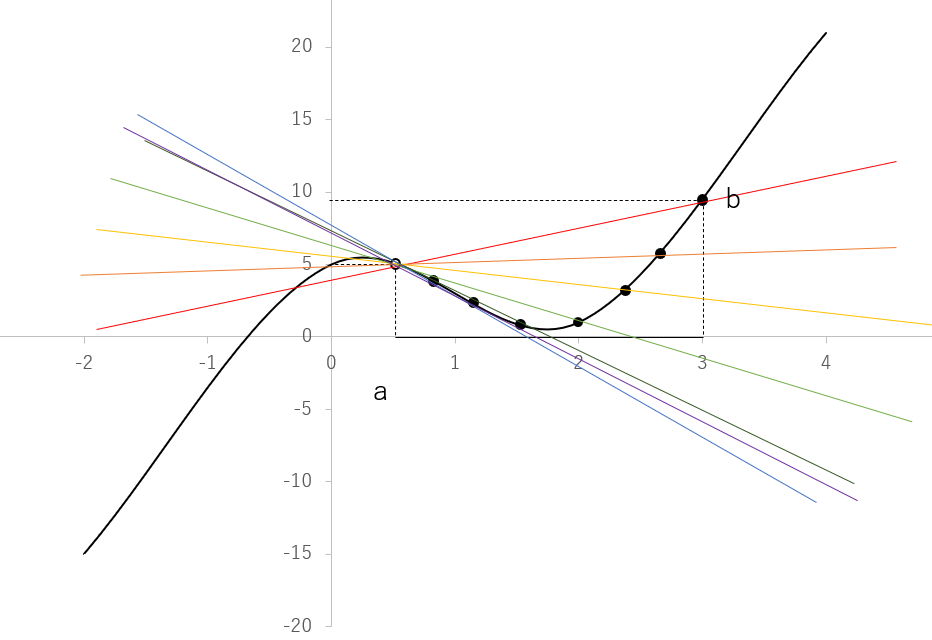
\includegraphics[scale=0.5]{img/QuuNote/differentialCoefficieant_Graph.png}
                \caption{点$b$を徐々に近づけた場合の直線の変化}
            \end{figure}

            この図を見ると$b$が$a$に近づくにつれて、二点を結んだ直線も点$a$の\textbf{接線}に近づいていることがわかる。
            つまり$x=a$における微分係数は点$a$の接線の傾きを表している。
        \clearpage
        \subsection{微分可能性と連続性}
            今度は関数が$f(x)$が$x=a$で微分可能であることと連続であることの違いについて考えていこう。
            一見するとこれら二つは同値であるかのように見える。\footnote{昔の数学者たちの間でも長らく連続関数は明らかに微分可能と考えられていたらしい。だからこそ「エルミートの怪物」
            のような連続なのにいたるところで微分不可能な関数が発見されたときは、数学界に大きな衝撃を与えたそうだ。\\参考サイト:\url{http://allneedislove380.blog61.fc2.com/blog-entry-291.html}}
            実際初等関数は連続である区間についてすべて微分可能である。では初等関数ではない関数である$y=|x|$で考えてみよう。
            もちろん$x>0$では$y=x$、$x<0$では$y=-x$であるので、微分可能である。(実際に試すとよい)
            しかし$x=0$においては微分可能ではない。\footnote{幾何学的に言えば接線が二本引けてしまうことが理由となる。つまり微分可能性とはその点においてただ一つ接線が引けることと理解できる。\label{微分可能性の幾何学的意味}}それを今から示す。

            微分可能であることは、右方微分係数と左方微分係数が一致すればよいことであるが
            \begin{equation}
                \frac{|0+h|-|0|}{h}=\frac{|h|}{h}
            \end{equation}
            なので、
            \begin{align}
                y'(+0)&=\lim_{h\to +0}\frac{|h|}{h}=\lim_{h\to+0}\frac{h}{h}=1\\
                y'(-0)&=\lim_{h\to -0}\frac{|h|}{h}=\lim_{h\to -0}\frac{-h}{h}=-1
            \end{align}
            となり右方微分係数と左方微分係数が一致しない。したがって$y=|x|$は微分可能ではない。
            しかし$x=0$で連続ではないので、$y=|x|$は連続であるが微分可能でない関数であることがわかる。

            では逆に$f(x)$が$x=a$で微分可能であるときはどうであろうか。$f(x)$が$x=a$で微分可能であるとき
            \begin{equation}
                \lim_{h\to 0}(f(a+h)-f(a))=\lim_{h\to 0}\frac{f(a+h)-f(a)}{h}\cdot h=\lim_{h\to 0}f'(a)\cdot h=0 
            \end{equation}
            また、$\displaystyle \lim_{h\to 0}(f(a+h)-f(a))=\lim_{h\to 0}f(a+h)-\lim_{h\to 0}f(a)=\lim_{h\to 0}f(a+h)-f(a)$なので、
            \begin{equation}
                \lim_{h\to 0}f(a+h)=f(a)
            \end{equation}
            が成り立つ。$h=b-a$であったことを思い出すと、$h\to 0$のとき$b\to a$なので
            \begin{equation}
                \lim_{b\to a}f(b) = f(a)
            \end{equation}
            つまり$x=a$で$f(x)$は連続の条件を満たす。\\\\
            \noindent
            以上をまとめると\fbox{$f(x)$が$x=a$で微分可能$\Rightarrow$$f(x)$は$x=a$で連続}である。 \\

            ちなみに、$x=a$で$f(x)$が不連続である場合は、対偶を取ればわかるように微分可能ではない。これは微分係数の定義からもわかる。
        \clearpage
        \subsection{導関数の定義}
            関数$f(x)$の微分係数は$f'(a)$であり、これは$x=a$の点において$y=f(x)$上の接線の傾きを意味していることは前回学んだ。
            では次に任意の$x$の値に対して$f(x)$の接線の傾きを返す関数を考えてみよう。この間数は以下のように定義できる。
            \begin{equation}
                f'(x)=\lim_{h\to 0}\frac{f(x+h)-f(x)}{h}
            \end{equation}
            このような関数$f'(x)$を$f(x)$の\textbf{導関数}という。$x=a$のときの導関数の値が$f'(a)$であり、これは$x=a$の微分係数である。

            導関数には以下のような書き方がある。
            \begin{equation}
                \frac{dy}{dx},\quad\frac{df}{dx},\quad y',\quad f'(x),\quad\frac{d}{dx}y,\quad\frac{d}{dx}f(x),\quad D_xf(x),\quad Df(x)
            \end{equation}
            このうち$\frac{d}{dx}$\footnote{読み方は分子から。「でぃーわいでぃーえっくす」など。}の書き方はライプニッツ、$f',y'$の書き方はラグランジュによるものである。$D_x,D$はコーシーによる。
            ライプニッツの書き方は導関数の意味が明瞭であるが書く際に場所を取ってしまったりするので簡潔なラグランジュの書き方も使われる。(コーシーの書き方は演算子であることが明瞭である気がする。)このノートはどちらもその
            場合に応じて使い分けていく。
            ちなみに、変数が時間である場合など、物理関係では$\dot{x}(t)$などとして表すこともある。これはニュートンの書き方である。\\

            試しに、$f(x)=x$の導関数を求めてみる。
            \begin{equation}
                f'(x)=\lim_{h\to 0}\frac{f(x+h)-f(x)}{h}=\lim_{h\to 0}\frac{(x+h)-x}{h}=1
            \end{equation}
            したがって、$f(x)=x$の導関数は$f'(x)=1$であることがわかる。これは定数関数であるので$x$の値によらない。
            つまり$y=x$はどの点でも傾きが同じであることがわかる。実際グラフを想像すれば直線で傾きは一定である。\\

            一般に$f,g$が微分可能、$a=定数$であるとき以下の公式が成り立つ。
            \begin{alignat}{3}
                &(a)' &&= 0\\
                &(a f(x))' &&= af'(x)\\
                &(f(x)\pm g(x))' &&=f'(x)\pm g'(x)
            \end{alignat}
            どれも定義からすぐに導出できる。気になる人は試してみてほしい。
        \clearpage
        \basicquestion 以下の問いに答えよ。

            \paragraph{問1}次の関数の(\hspace{2mm})内の区間での平均変化率を求めよ。
            \begin{alignat*}{2}
                &(1)y=x^2+1 &&(x=1\to 3)\\
                &(2)y=x^3+x^2+x+1 &&(x=-1\to 1)\\
                &(3)y=\sin x &&(x=\frac{\pi}{6}\to\frac{\pi}{3})
            \end{alignat*}

            \paragraph{問2}次の関数を微分せよ。\\
            \noindent
            $(1)y=x+1$\hspace{5mm}
            $(2)y=5$\hspace{5mm}
            $(3)y=x^3$\hspace{5mm}
            $(4)y=ax+b$\hspace{5mm}
            $(5)y=a(x+p)^2+q$

            
            \paragraph{問3}$y=\sqrt{x}\hspace{1mm}(x\geq 0)$が微分可能であるか調べよ。

            \paragraph{問4}以下の式を証明せよ。
            \begin{equation*}
                \frac{d}{dx}(af(x))=a\frac{d}{dx}f(x)
            \end{equation*}
            ただし、$f(x)$が微分可能とする。
        \clearpage
        \section{導関数の計算}
            \subsection{基礎的な関数の導関数}
                \noindent
                ここでは初等関数の基礎的な関数$x^n,\sin x,e^x,\log x$などの導関数を求めていく。\\

                まず、$e^x$から考えてみよう。ひとまず定義に従えば
                \begin{equation}
                    \lim_{h\to 0}\frac{e^{x+h}-e^{x}}{h}=e^x\lim_{h\to 0}\frac{e^h-1}{h}
                \end{equation}
                と変形できる。そこで、出てきた極限について逆数をとり$t=e^h-1$とおいて計算していく。
                \begin{equation}
                    \lim_{h\to 0}\frac{h}{e^h-1}=\lim_{t\to 0}\frac{\log(t+1)}{t}=\lim_{t\to 0}\log(1+t)^\frac{1}{t}
                \end{equation}
                と変形できるので、$e$の定義式(\ref{eq:define_e})より真数は$e$となる。したがってこの極限は$1$となるので
                \begin{equation}
                    (e^x)'=e^x \cdot \lim_{h\to 0}\frac{e^h-1}{h}=e^x \cdot 1 =e^x
                \end{equation}
                つまり$e^x$は\underline{微分しても形が変わらない}のである。
                また、この結果を使えば一般の指数関数$a^x$の導関数も簡単に求まる。$(e^{ax})'=ae^{ax}$が成り立つ(演習問題)ことから
                \begin{equation}
                    (a^x)'=(e^{\log(a^x)})'=(e^{x\log a})'=e^{x\log a}\log a=a^x\log a
                \end{equation}

                つぎに、$\log x$について考えてみる。これも定義に従って
                \begin{equation}
                    \lim_{h\to 0}\frac{\log(x+h)-\log x}{h}=\lim_{h\to 0}\frac{\log\left(\frac{x+h}{x}\right)}{h}=\lim_{h\to 0}\log\left(1+\frac{h}{x}\right)^\frac{1}{h}
                \end{equation}
                ここで$t=\frac{h}{x}$と置けば
                \begin{equation}
                    \lim_{t \to 0}\log(1+t)^\frac{1}{xt}=\lim_{t\to 0}\frac{\log(1+t)^\frac{1}{t}}{x}=\frac{\log(e)}{x}=\frac{1}{x}
                \end{equation}
                と求まる。

                次に、$x^n$で求めてみよう。ただし$n$は自然数であるとする。一般に、
                \begin{equation}
                    (x+a)^n=x^n+{}_nC_1ax^{n-1}+{}_nC_2a^2 x^{n-2}+\cdots +{}_nC_ma^{m}x^{n-m}+\cdots {}_nC_1a^{n-1}x+a^n\quad(\text{\textbf{二項定理}})
                \end{equation}
                が成り立つので
                \begin{alignat}{1}
                    (x^n)'&=\lim_{h\to 0}\frac{(x+h)^n-x^n}{h}=\lim_{h\to 0}\frac{{}_nC_1hx^{n-1}+{}_nC_2h^2 x^{n-2}+\cdots +{}_nC_mh^{m}x^{n-m}+\cdots +{}_nC_1h^{n-1}x+h^n}{h}\\
                    &=\lim_{h\to 0} {}_nC_1 x^{n-1}+(h\text{についての多項式})=nx^{n-1}
                \end{alignat}
                要するに$x^n$の微分は\underline{肩をおろして1を引く}のである。
                \clearpage
                最後に$\sin x$の導関数を求めてみよう。こちらも定義通りに計算して
                \begin{equation}
                    (\sin x)'=\lim_{h\to 0}\frac{\sin(x+h)-\sin x}{h}=\lim_{h\to 0}\frac{2\cos(\frac{2x+h}{2})\sin(\frac{h}{2})}{h}=\lim_{h\to 0}\cos (x+\frac{h}{2})\cdot \lim_{h\to 0}\frac{\sin\frac{h}{2}}{\frac{h}{2}}=\cos x
                \end{equation}
                最後の極限は式\ref{eq:limit of sin/x}を利用した。\\

                これで基礎となる関数の導関数はほとんど導出できた。以下公式としてまとめる。一部導出していないものもあるが演習問題で導出する。これくらいは後々の計算のためにも覚えておくとよい。

                \begin{screen}
                    \begin{alignat*}{2}
                        &(x^n)'=nx^{n-1} && (a^x)'=a^x\log a\\
                        &(e^x)'=e^x && (\log x)'=\frac{1}{x}\\
                        &(\sin x)'=\cos x \quad&& (\cos x)'=-\sin x
                    \end{alignat*}
                \end{screen}
            \clearpage
            \subsection{積の微分}
                今度は 関数同士の積について、公式を導出してみよう。$f,g$は微分可能であるとする。このとき、
                \begin{equation}
                    (f(x)g(x))'=\lim_{h\to 0}\frac{f(x+h)g(x+h)-f(x)g(x)}{h}
                \end{equation}
                である。当然このままでは計算できないので少し式をいじってあげよう。仮定より分子にどうにかして$f(x+h)-f(x)$もしくは$g(x+h)-g(x)$
                を作れないか考えてみる。そこで分子に$-f(x+h)g(x)+f(x+h)g(x)=0$を加えてあげると
                \begin{equation}
                    \frac{f(x+h)(g(x+h)-g(x))+g(x)(f(x+h)-f(x))}{h}=\frac{f(x+h)(g(x+h)-g(x))}{h}+\frac{g(x)(f(x+h)-f(x))}{h}
                \end{equation}
                とできる。あとは$f,g$が微分可能であるので$h\to  0$の極限を取れば
                \begin{equation}
                    (f(x)g(x))'=f(x)g'(x)+f'(x)g(x)\label{eq:積の微分公式}
                \end{equation}
                こうして積の微分公式が得られた。では、この公式を用いて$\displaystyle y=x^{-n}=\frac{1}{x^{n}}$の導関数も求めてみよう。
                \begin{equation}
                    (1)'=\left(\frac{x^n}{x^{n}}\right)'=nx^{n-1}\cdot \frac{1}{x^{n}}+x^n\cdot \left(\frac{1}{x^n}\right)'=\frac{n}{x}+x^{n}y'=0
                \end{equation}
                であるため、$y'=$の形に整理すれば
                \begin{equation}
                    y'=\frac{-n}{x^{n+1}}=(-n)\cdot x^{(-n)-1}\label{eq:積微分による1/x^nの微分}
                \end{equation}
                つまり、任意の整数について$(x^n)'=nx^{n-1}$が成り立つことが示せた。\footnote{この例は積の微分公式を使う練習としてはあまり適していない。商の微分を用いるか合成関数の微分法を用いることで見通しよく求められる。}\\

                もう少し簡単な問題で積の微分公式を使う練習をしてみよう。
                \paragraph{例題}$y=x\sin x$のとき$y'$を求めよ。\\
                $f=x,g=\sin x$とおいて式\ref{eq:積の微分公式}を適応すると$f'=1,g'=\cos x$だから
                \begin{equation}
                    y'=fg'+f'g=x\cos x+\sin x
                \end{equation}
                と求まる。
            \clearpage
            \subsection{商の微分}
                積の微分について考えたら次は商の微分についても考えたくなるものである。商の微分公式について以下にのべる。
                \begin{equation}
                    \left(\frac{f(x)}{g(x)}\right)'=\frac{f'(x)g(x)-f(x)g'(x)}{\left\{g(x)\right\}^2}\label{eq:商の微分公式}
                \end{equation}
                もちろん$f,g$は微分可能であり$g(x)\neq 0$であるとする。頭の痛くなる形をしていて、覚えるのに苦労しそうである。
                覚え方は人によってさまざまだろうが、例えば「分子は積の微分の符号反転で分母は二乗する」という覚え方もある。導出については
                演習問題とする。

                商の微分について$f=1$の特別な場合を知っておくと計算が早くなることがある。試しに公式に代入してみると
                \begin{equation}
                    \left(\frac{1}{g}\right)'=\frac{0\cdot g-1\cdot g'}{g^2}=-\frac{g'}{g^2}
                \end{equation}
                となる。最後の符号を忘れないように注意しよう。ここまで覚える必要はないが知っておけば多少楽できる。\\

                ではこれを使って$y=x^{-n}$の導関数を導出してみよう。$f=1,g=x^n$として公式に代入すればよい。
                \begin{equation}
                    y'=-\frac{(x^n)'}{(x^n)^2}=-\frac{nx^{n-1}}{(x^n)^2}=-\frac{n}{x^{n+1}}=(-n)\cdot x^{(-n)-1}
                \end{equation}
                となり、式\ref{eq:積微分による1/x^nの微分}と同じ結果が得られた。こちらの方が自然な導出である。

                次に$y=\tan x$の導関数を導出してみよう。この関数は$\sin x$などと違って定義から計算すると骨が折れる。しかし、商の微分公式を用いれば
                \begin{equation}
                    y'=\left(\frac{\sin x}{\cos x}\right)'=\frac{\cos^2 x-(-\sin^2 x)}{\cos^2 x}=\frac{1}{\cos^2 x}
                \end{equation}
                と楽に導出できる。
            \clearpage
            \subsection{合成関数の微分}
                では次に合成関数の微分について考えてみる。$y=f(g(x))$として考えてみる。このとき
                \begin{equation}
                    y'=\lim_{h\to 0}\frac{f(g(x+h))-f(g(x))}{h}=\lim_{h\to 0}\frac{f(g(x+h))-f(g(x))}{g(x+h)-g(x)}\cdot \frac{g(x+h)-g(x)}{h}
                \end{equation}
                であるので、$h'=g(x+h)-g(x)$と置けば、$h\to 0$で$h'\to0$なので、
                \begin{equation}
                    \lim_{h'\to 0}\frac{f(g(x)+h')-f(g(x))}{h'}\cdot \lim_{h\to 0}\frac{g(x+h)-g(x)}{h}=f'(g(x))\cdot g'(x)
                \end{equation}
                となる。$u=g(x)$とおいてこれをライプニッツの記号で書けば
                \begin{equation}
                    \frac{dy}{dx}=\frac{dy}{du}\frac{du}{dx}\label{eq:合成関数の微分}
                \end{equation}
                こうすれば`形式的に'約分しているように見ることができる。ちなみにこの合成関数の微分の公式を\textbf{チェイン・ルール}という。
                
                合成関数の微分公式を用いれば一般の$m$について$(x^m)'=mx^{m-1}$が証明できる。それを今から示す。\footnote{これは対数微分法でも示せる。そもそも対数微分法も今回のやり方も本質的には同じである。}
                \begin{equation}
                    (x^m)'=(e^{\log x^m})'=(e^{m\log x})'=e^{m\log x}\cdot (m\log x)'=x^{m}\cdot \frac{m}{x}
                \end{equation}
                と計算できるので、
                \begin{equation}
                    (x^m)'=mx^{m-1}
                \end{equation}
                
                ほかにも$(2x+1)^5$を微分するとき、通常なら展開して項別微分する必要があるが、合成関数を用いれば
                \begin{equation}
                    \left\{(2x+1)^5\right\}'=5(2x+1)^4\cdot (2x+1)'=10(2x+1)^4
                \end{equation}
                と非常に簡単に求められる。より一般的には
                \begin{equation}
                    (f(ax+b))'=af'(ax+b)
                \end{equation}
                である。
            \clearpage
            \subsection{逆関数の微分}
                前回までで和・差・積・商のすべての場合について、微分の公式を導入した。これさえあればどんな関数でも微分できそうであるが、実はそうではない。
                例えば$\arcsin x$は、$\sin x$の逆関数であること以外何も関数についてわかっていない。このような関数の微分について考えよう。

                まず、$f(x)$について、逆関数を$y=f^{-1}(x)$と表すことにすれば、導関数の定義より
                \begin{equation}
                    \lim_{h\to 0}\frac{f^{-1}(x+h)-f^{-1}(x)}{h}
                \end{equation}
                ここで$y=f^{-1}(x)$と置くと、$x=f(y)$である。また、$Y=f^{-1}(x+h)$と置けば$x+h=f(Y)$である。したがって$h=f(Y)-f(y)$である。$h\to 0$のとき$Y\to y$だから$h'=Y-y$と置けば$h'\to 0$である。
                \begin{equation}
                    \lim_{h'\to 0}\frac{h'}{f(y+h')-f(y)}=\lim_{h'\to 0}\frac{1}{\displaystyle\frac{f(y+h')-f(y)}{h'}}
                \end{equation}
                ここで$f(x)$が微分可能であるとすれば、この極限は収束して
                \begin{equation}
                    \frac{dy}{dx}=\frac{1}{\displaystyle\frac{dx}{dy}}\label{eq:逆関数の微分公式}
                \end{equation}
                となる。これが逆関数の微分公式である。形式的には$dy,dx$の分子と分母を入れ替えた形と一致する。\\

                ではこの公式を用いて件の$\arcsin x$を求めてみることにしよう。$y=\arcsin x$とすれば当然$x=\sin y$であるから、
                \begin{equation}
                    \frac{dy}{dx}=\frac{1}{\displaystyle\frac{dx}{dy}}=\frac{1}{\displaystyle\frac{d}{dy}\sin y}=\frac{1}{\cos y}=\frac{1}{\sqrt{1-\sin^2 y}}=\frac{1}{\sqrt{1-x^2}}
                \end{equation}
                と求まった。つぎに$y=\log x$について、公式を適用してみよう。逆関数が$e^x$であることに注意すれば
                \begin{equation}
                    \frac{dy}{dx}=\frac{1}{\frac{d}{dy}e^{y}}=\frac{1}{e^y}=\frac{1}{x}
                \end{equation}
                となり、公式が正しいことも確認できる。
            \clearpage
            \subsection{微分}
                ここでは微分という概念について述べる。突然だが微分可能な関数$f$について$y=f(x)$のグラフを考えてみる。この時グラフ上の点$(x,y)$
                は、必ず接線を持つはずである。\footref{微分可能性の幾何学的意味}このとき、その接線上の点$(X,Y)$について$dx=X-x,dy=Y-y$となるような
                座標の変動$dx,dy$を定義してあげると
                \begin{equation}
                    dy=f'(x)dx
                \end{equation}
                は、点$(x,y)$の接線の方程式と全く同じものであることがわかる。この時$dx=\Delta x$とすると、
                グラフ上の座標の変動$\Delta y$は必ずしも$dy$と等しくはならない。このような$dx,dy$をそれぞれ$x,y$の\textbf{微分}という。\\

                これらの意味するところについて述べたいのはやまやまだが、ここでは記号的な話にのみ焦点を当てる。形式的な話であるので得られた結果が正しい可能性はないし、
                そもそもここからすべての導関数が導出できるわけではないだろうが、便利なので紹介する。

                まずは、演算の規則について、次の三つがある。
                \begin{enumerate}
                    \item $dy=f'(x)dx$
                    \item $d(u\pm v)=du\pm dv$
                    \item $d(uv)=vdu+udv$
                \end{enumerate}
                
                これを用いて一つ導関数を求めてみよう。例えば陰関数$F(x,y)=x^2+y^2-r^2=0$について、$\frac{dy}{dx}$を求めてみることにする。まず、$x,y$を両辺に分け、それぞれ$d$(ディー)して
                \begin{equation}
                    d(x^2-r^2)=d(y^2)
                \end{equation}
                演算の規則2より、$d(x^2-r^2)=d(x^2)-d(r^2)$と分けられる。この時、$r$は$x,y$によらないと考えているので$d(r^2)=0$である。よって、
                \begin{equation}
                    2xdx=2ydy
                \end{equation}
                式を変形すると、
                \begin{equation}
                    \frac{dy}{dx}=\frac{x}{y}
                \end{equation}
                となる。まるで魔法にかけられたみたいにあっさり求まってしまったが、この結果は正しいのだろうか?試しに$y>0$として元の式を変形すると$y=\sqrt{r^2-x^2}$となる。
                このとき、$x$微分すると
                \begin{equation}
                    \frac{dy}{dx}=\frac{x}{\sqrt{r^2-x^2}}=\frac{x}{y}
                \end{equation}       
                と確かに一致することがわかる。        
            \clearpage
            \basicquestion 以下の問いに答えよ。
            
                \paragraph{問1}以下の関数の導関数を求めよ。\\
                $(1)y=x^2+1$\hspace{3mm}
                $(2)y=\cos x+\sin x$\hspace{3mm}
                $(3)y=\log 2x$\hspace{3mm}
                $(4)y=\cos^{-1}x$\hspace{3mm}
                $(5)y=e^{\tan x}$\hspace{3mm}
                $(6)y=e^{x^2}\cos 2x$\\
                $\displaystyle(7)y=\log(x+\sqrt{x^2+1})$\hspace{3mm}
                $(8)y=f^{-1}(x)\quad (f(x)=x^4)$

                \paragraph{問2}以下を示せ。\\
                (1)商の微分公式(\ref{eq:商の微分公式})を示せ。\\
                (2)$(e^{ax})'=ae^{ax}$を導関数の定義から導出せよ。\\
                (3)$\cos x$の導関数を$\sin^2 x+\cos ^2 x=1$の関係を利用して導出せよ。ただし$\cos x\neq 0$であるとする。

                \paragraph{問3}以下の関数の導関数を工夫して求めよ。\\{\scriptsize ヒント:(1)(2)両辺対数を取るか$e^{\log f(x)}$の形にせよ。(3)普通に解いてもよいが$x=\tan \theta$と置いて合成関数の微分公式を用いると楽に出せる。}\\
                $\displaystyle(1)y=\sqrt[3]{\frac{x^2+1}{(x+1)^2}}\quad(x>-1)$\hspace{3mm}
                $(2)y=x^x$\hspace{3mm}
                $\displaystyle(3)y=\sin^{-1}\frac{x}{\sqrt{1+x^2}}$

                \paragraph{問4}双曲線関数について、$\sinh x,\cosh x$の導関数を導出せよ。

                \paragraph{問5}以下の公式について、後の問いに答えよ。
                \begin{eqnarray}
                    \sin\alpha\cos\beta=\frac{1}{2}\left\{\sin(\alpha+\beta)+\sin(\alpha+\beta)\right\}\label{eq:和積の公式sinαcosβ}
                \end{eqnarray}
                \begin{enumerate}\setcounter{enumi}{0}\renewcommand{\labelenumi}{(\arabic{enumi})}
                    \item 公式(\ref{eq:和積の公式sinαcosβ})を示せ。
                    \item 公式(\ref{eq:和積の公式sinαcosβ})の両辺を$\alpha$微分せよ。
                    \item 公式(\ref{eq:和積の公式sinαcosβ})の両辺を$\beta$微分せよ。
                \end{enumerate}
                
            \clearpage
            \section{微分法の応用}
                \subsection{関数の増減}
            \clearpage
            \section{微分法諸定理}


            
            

                
    \clearpage

    \part{積分$\int$}

    \clearpage
    \part{無限級数$\sum$}
    \clearpage
    \part{終わりに}
        このノートでは、(高専2年生で扱う)一変数の微分積分+無限級数について主に扱った。ここに書いてあることが大抵わかれば、
        高専2年の数学程度は楽勝であるはずである。数学書も入門書レベルなら読めるはずである。(...読めてほしい。)
        
        さて、何度も言うようにここでは``一変数''関数の微分積分についてのみ扱った。つまり多変数関数についての微分積分は言及してないわけである。
        多変数の微分積分は一変数と違うところが多々ある。例えば、二変数関数について極限を取るときに、一変数の場合はx軸上での近づき方のみ考えていたが
        二変数関数となるとxy`平面'での近づき方を考える必要がある。つまり、x軸上,y軸上に沿って近づく場合以外に$x,y$が同時に動く場合も考えなければならない。
        微分についても多変数の場合は\textbf{偏微分}という名前になり、記号として$\partial$を用いるようになる。積分についても、例えば二変数の場合は積分領域が
        平面となる。

        多変数の微分積分の先にはどんな学問があるのかという話だが、主に「微分方程式」「複素関数」「ベクトル解析」「フーリエ解析」があげられる。\\

        話は変わるが、このノートを読んでもっと厳密なことを勉強したい、先のことを勉強したい人のためにこのノートを作る際に参考にした書籍を一部上げることにする。
        \begin{enumerate}\setcounter{enumi}{0}\renewcommand{\labelenumi}{(\arabic{enumi})}
            \item \href{https://www.iwanami.co.jp/book/b482316.html}{\textbf{理工系の数学入門コース 新装版 微分積分}}\\ノートで紹介した内容に加えて多変数の微分積分まで扱っている。私が初めて読んだ本でもあり、初学者でも読みやすくなっている。
            このノートの大部分はこの本に影響されているといっても過言ではない。これの姉妹図書である演習版も併用するとなおよい。コラムも面白い。
            \item \href{https://www.iwanami.co.jp/book/b265489.html}{\textbf{解析概論}}\\言わずと知れた解析学の名著。著者は高木貞二。理工学生は一度はこの本を読むべきとまで言われる。実際読んでみると、確かにわかりやすい。
            私自身全部読み切れてはいないが、(それでも)一見の価値ありだと思われる。この本から学ぶことも多かった。
            \item \href{https://www.dainippon-tosho.co.jp/college_math/differential1.html}{\textbf{新 微分積分}I \textbf{改訂版}}\\高専2年生で使われる教科書。一年生の内容から円滑に理解できるように工夫されている。
            しかし、極限の定義があいまいであったり、積分が公式ゲーみたいになっているところはあまりよくない。
            \item (準備中)
        \end{enumerate}
    \clearpage
    \section{模範解答}
        次ページから問題の模範解答を示す。
        \clearpage\color{red}
        \subsection{前提知識 基本問題解答}
            \basicanswer 
                \paragraph{問1}以下の主張のうち正しいものには〇を、間違っているものには×をつけよ。
                \begin{enumerate}
                    \item $\sqrt{9}$は無理数である。
                    \item 有理数は全て分子分母が整数である分数の形で表せる。
                    \item $i$は複素数である。
                    \item 有理数の集合は$\mathbb{Q}$として表し、無理数の集合は$\mathbb{N}$で表す。
                    \item 自然数全体の集合(区間)は$(0,\infty]$である。
                \end{enumerate}
                正しいのは1,2,3、間違っているのは4,5
                \paragraph{問2}以下の区間について、数直線上に示せ。もし数直線上に記されていない数字が出てくる場合はそれも記載せよ。
                    \begin{figure}[h]
                        \centering
                        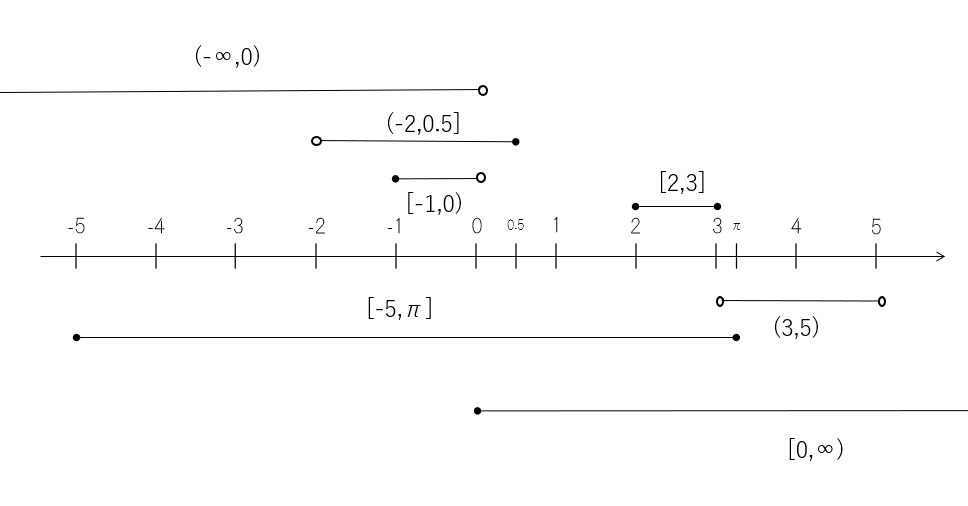
\includegraphics[keepaspectratio,scale=0.6]{img/QuuNote/kihonmondaikaitouzu_1.png}
                        \caption{数直線}
                    \end{figure}

                    $1.\quad [2,3]$\hspace{3mm}
                    $2.\quad (3,5)$\hspace{3mm}
                    $3.\quad [-5,\pi]$\hspace{3mm}
                    $4.\quad (-2,0.5]$\hspace{3mm}
                    $5.\quad [-1,0)$\hspace{3mm}
                    $6.\quad (-\infty,0)$\hspace{3mm}
                    $7.\quad [0,\infty)$\hspace{3mm}
            \clearpage
            \basicanswer
                \paragraph{問1}次の関数が偶関数か奇関数かを判別せよ。

                \noindent
                (1)偶\hspace{3mm}
                (2)奇\hspace{3mm}
                (3)奇\hspace{3mm}
                (4)偶\hspace{3mm}
                (5)奇\hspace{3mm}
                (6)どちらでもない\hspace{3mm}
                (7)偶\hspace{3mm}
                (8)奇

                \paragraph{問2}以下の等式を証明せよ。

                \noindent
                $(1)$加法定理で$\alpha=\beta=x$と置く。$\sin(2x)=\sin x\cos x+\cos x\sin x=2\sin x\cos x$\hspace{1mm}$\cos 2x$も同様。\\
                $(2)$倍角の公式より、$\cos 2x=\cos^2 x-\sin^2 x=1-2\sin^2 x$変形して$x$に$\frac{x}{2}$を代入すれば半角の公式が得られる。$\cos^2 \frac{x}{2}$も同様。\\
                $\displaystyle(3)\sinh(x+y)=\frac{e^{x+y}-e^{-(x+y)}}{2}=\frac{e^{x+y}-e^{x-y}+e^{x-y}-e^{-x-y}}{2}=\frac{e^{x}(e^{y}-e^{-y})+e^{-y}(e^x-e^{-x})}{2}=e^x\sinh y+e^{-y}\sinh x=2\cosh x\sinh y -e^{-x}\sinh y+2\cosh y\sinh x -e^{y}\sinh x$\\
                ここで$\displaystyle e^{-x}\sinh y+e^{y}\sinh x=\frac{e^{y-x}-e^{-y-x}}{2}+\frac{e^{x+y}-e^{y-x}}{2}=\sinh(x+y)$である。\\
                よって、$\displaystyle \sinh (x+y)=2\cosh x\sinh x+2\cosh y\sinh x-\sinh (x+y)\to \sinh(x+y)=\cosh x\sinh x+\cosh y\sinh x$となる。$\cosh (x+y)$についても同様。
                
                \paragraph{問3}以下の値を求めよ。

                \noindent
                $(1)0$\hspace{3mm}
                $(2)\frac{\pi}{6}$\hspace{3mm}
                $(3)0$\hspace{3mm}
                $(4)3$\hspace{3mm}
                $(5)0$\hspace{3mm}
                $(6)1$\hspace{3mm}
                $(7)\frac{\pi}{2}-\cos\log 3\sin\log 2$
                
                \paragraph{問4}$I=271\times 314$と置けば、$\log_{10} I=\log_{10}2.71+\log_{10}3.14+4$である。よって、$\log_{10}I=4.9315$より$I=10^{4.9315}\simeq 85408$
                
                \paragraph{問5}$t=\tan\frac{x}{2}$とするとき、$\sin x,\cos x,\tan x$をそれぞれ$t$を用いた式で表せ。
                \begin{align*}
                    \sin x &=2\sin \frac{x}{2}\cos \frac{x}{2}=\frac{2\tan\frac{x}{2}}{\frac{1}{\cos^2\frac{x}{2}}}=\frac{2t}{1+t^2}\\
                    \cos x &=\cos^2 \frac{x}{2} -\sin^2 \frac{x}{2}=\frac{1-\tan^2\frac{x}{2}}{\frac{1}{\cos ^2\frac{x}{2}}}=\frac{1-t^2}{1+t^2}\\
                    \tan x &=\frac{\sin x}{\cos x}=\frac{\displaystyle\frac{2t}{1+t^2}}{\displaystyle\frac{1-t^2}{1+t^2}}=\frac{2t}{1-t^2}
                \end{align*}
            \clearpage
            \basicanswer 
            
                \paragraph{問1}以下の数列の一般項を示し、それらが収束するかどうか答えよ。\\
                $(1)\frac{n+1}{n}=1+\frac{1}{n}$収束する\hspace{3mm}
                $(2)\frac{1}{3^n}$収束する\hspace{3mm}
                $(3)(-1)^{n+1}$発散する\hspace{3mm}
                $(4)a+(n-1)d$発散する

                \paragraph{問2}仮定より$\displaystyle |a-a_n|<\frac{\varepsilon}{2}\quad(n>N_1),|b-b_n|<\frac{\varepsilon}{2}\quad(n>N_2)$となる$N_1,N_2$が存在する。ここで、$N_1,N_2$のうち大きい方をとり
                \footnote{ここで大きい方を取ることで、必ず仮定の条件を満たす。例えば$N_1>N_2$であるとき$N=N_1$と取れば、どちらの数列に対しても$\ldots<\frac{\varepsilon}{2}$となるが、$N=N_2$と取ってしまうと$N_1>n>N_2$であるような$n$に対して$|a-a_n|<\frac{\varepsilon}{2}$が保証できないのである。}
                、それを$N=\max(N_1,N_2)$と置けば$n>N$のとき
                \begin{equation*}
                    |(a+b)-(a_n+b_n)|=|(a-a_n)+(b-b_n)|\leq |a-a_n|+|b-b_n|<\frac{\varepsilon}{2}+\frac{\varepsilon}{2}=\varepsilon
                \end{equation*}
                となるような$N$が存在する。よって、証明完了。

                \paragraph{問3}以下計算せよ。\\

                \noindent
                $(1)2$\hspace{3mm}
                $(2)4\pi^2$\hspace{3mm}
                $(3)0$\hspace{3mm}
                $(4)2$\hspace{3mm}
                $(5)0$\hspace{3mm}
                $(6)-1$\hspace{3mm}
                $(7)\frac{1}{2}$\hspace{3mm}
                $(8)1$
                
                \paragraph{問4}次の関数が()内の点において連続であるかどうか調べよ。\\
                $(1)$連続\hspace{1mm}
                $(2)$連続\hspace{1mm}
                $(3)$連続\hspace{1mm}
                $(4)$不連続\hspace{1mm}
                $(5)$連続\\
                $(6)\displaystyle \lim_{x\to 0}f(x)=\lim_{x\to 0}x\sin\frac{1}{x}$に注意する。また、$-1\leq\sin\frac{1}{x}\leq 1$であるため、$-x\leq f(x) \leq x$
                ここで$x\to 0$の極限を取れば$x,-x\to 0$なのではさみうちの原理より$f(x)\to 0.$これは$f(0)=1$と一致しないので、\underbar{不連続}

                \paragraph{問5}方程式$\sin x=x$が区間$[0,\frac{\pi}{2}]$に実数解をもつかどうか調べよ。

                $x=0$で等号が成り立つので実数解は存在する。\\
                (補足)$\cos x=x$の場合でも実数解をもつか考えてみることにする。
                $f(x)=\cos x-x$と置くと、$f(x)$は$[0,\frac{\pi}{2}]$で連続であり
                \begin{equation*}
                    f(0)=1>0,\quad f\left(\frac{\pi}{2}\right)=-\frac{\pi}{2}<0
                \end{equation*}
                したがって中間値の定理より区間$[0,\frac{\pi}{2}]$に$\cos x=x$は実数解をもつ。
        \clearpage
        \subsection{微分法 基本問題解答}
        \clearpage
        \subsection{積分 基本問題解答}
        \clearpage
        \subsection{無限級数 基本問題解答}
        \clearpage
        \subsection{演習問題解答}
        \clearpage
        \color{black}

        \thispagestyle{fancy}
        \fancyhead{}
        \fancyfoot{\centerline{\hyperref[目次]{目次に戻る}}}

        \vspace{\stretch{1}}
        \begin{figure}
            \centering
            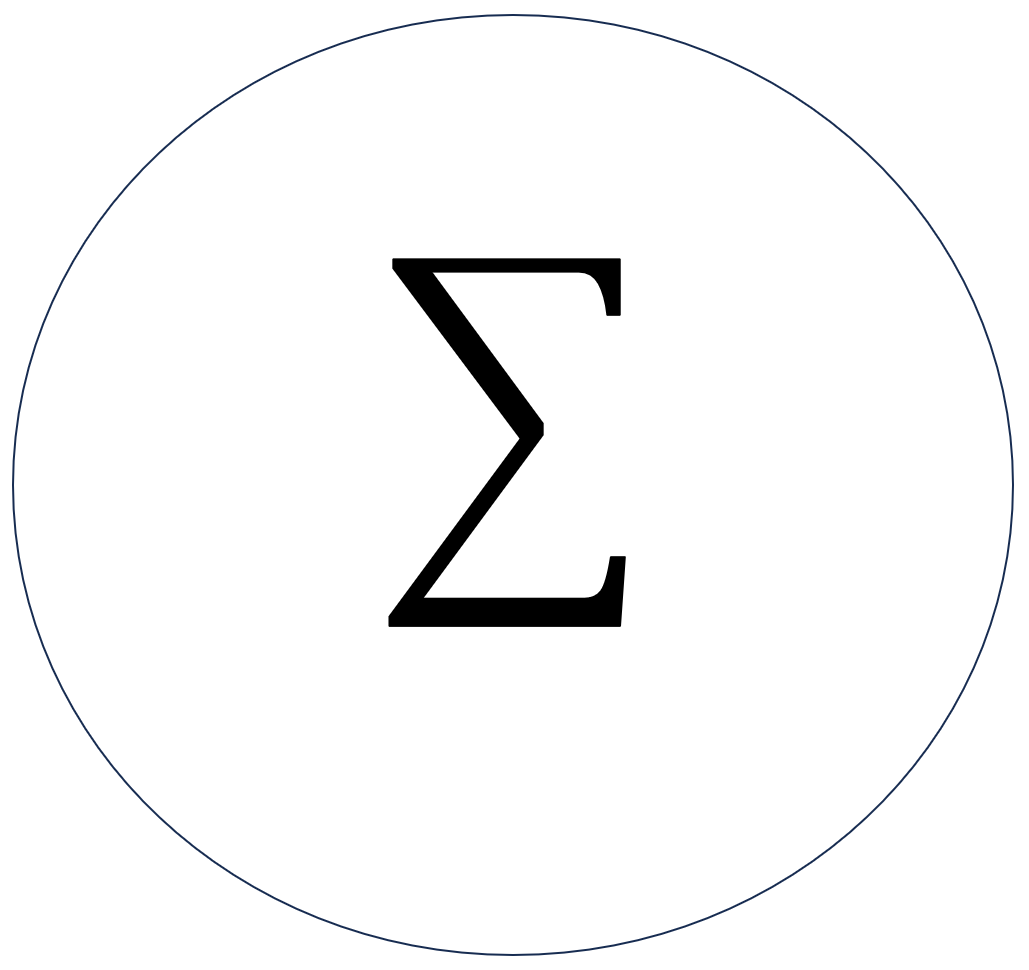
\includegraphics[scale=0.5]{img/QuuNote/icon.png}
        \end{figure}    
        \vspace{\stretch{1}}

        

\end{document}